\documentclass[12pt, a4paper, oneside]{report}

% ─── Packages ─────────────────────────────────────────────────────────────────
\usepackage[a4paper, top=3cm, bottom=3cm, left=3.5cm, right=2.5cm]{geometry}
\usepackage{setspace}
\usepackage{graphicx}
\usepackage{float}
\usepackage{amsmath, amssymb, bm}
\usepackage{booktabs}
\usepackage{array}
\usepackage{multirow}
\usepackage{xcolor}
\usepackage{listings}
\usepackage{caption}
\usepackage{subcaption}
\usepackage{hyperref}
\usepackage{fancyhdr}
\usepackage{natbib}
\usepackage{titlesec}
\usepackage{enumitem}
\usepackage{tabularx}
\usepackage{longtable}
\usepackage{mathtools}
\usepackage{microtype}
\usepackage{lmodern}
\usepackage[T1]{fontenc}
\usepackage{parskip}

% ─── Colours ──────────────────────────────────────────────────────────────────
\definecolor{navy}{RGB}{29,53,87}
\definecolor{accentblue}{RGB}{37,99,235}
\definecolor{codelightgray}{RGB}{248,249,250}
\definecolor{codekeyword}{RGB}{0,0,200}
\definecolor{codestring}{RGB}{163,21,21}
\definecolor{codecomment}{RGB}{100,116,139}

% ─── Hyperref ─────────────────────────────────────────────────────────────────
\hypersetup{
  colorlinks = true,
  linkcolor  = navy,
  citecolor  = accentblue,
  urlcolor   = accentblue,
  pdftitle   = {AI Football Scout v3: Predicting Transfer Success Through Player-Club Fit},
  pdfauthor  = {Victor Bomberna},
}

% ─── Typography ───────────────────────────────────────────────────────────────
\onehalfspacing
\setlength{\parskip}{6pt}

% ─── Headers ──────────────────────────────────────────────────────────────────
\pagestyle{fancy}
\fancyhf{}
\fancyhead[L]{\small\textcolor{navy}{\leftmark}}
\fancyhead[R]{\small\textcolor{navy}{\thepage}}
\renewcommand{\headrulewidth}{0.4pt}
\renewcommand{\headrule}{\hbox to\headwidth{\color{navy}\leaders\hrule height \headrulewidth\hfill}}

% ─── Chapter titles ───────────────────────────────────────────────────────────
\titleformat{\chapter}[display]
  {\normalfont\huge\bfseries\color{navy}}
  {\chaptertitlename\ \thechapter}{16pt}{\Huge}
\titlespacing*{\chapter}{0pt}{-10pt}{20pt}

\titleformat{\section}
  {\normalfont\Large\bfseries\color{navy}}
  {\thesection}{1em}{}
\titleformat{\subsection}
  {\normalfont\large\bfseries\color{navy!80}}
  {\thesubsection}{1em}{}

% ─── Code listings ────────────────────────────────────────────────────────────
\lstset{
  backgroundcolor = \color{codelightgray},
  basicstyle      = \ttfamily\small,
  keywordstyle    = \color{codekeyword}\bfseries,
  stringstyle     = \color{codestring},
  commentstyle    = \color{codecomment}\itshape,
  breaklines      = true,
  frame           = single,
  rulecolor       = \color{navy!30},
  numbers         = left,
  numberstyle     = \tiny\color{codecomment},
  showstringspaces= false,
  tabsize         = 4,
}

% ─── Custom commands ──────────────────────────────────────────────────────────
\newcommand{\fitscoreformula}{%
  \texttt{success\_score} = 0.35 \times m_{y1} + 0.30 \times gc_{y1} + 0.20 \times s_{2y} + 0.15 \times \phi
}

\graphicspath{{presentation_assets/}}

% ══════════════════════════════════════════════════════════════════════════════
\begin{document}

% ─── Title page ───────────────────────────────────────────────────────────────
\begin{titlepage}
\centering
\vspace*{2cm}
{\Huge\bfseries\color{navy} AI Football Scout v3 \par}
\vspace{0.5cm}
{\Large\color{navy!70} Predicting Transfer Success Through Player--Club Fit \par}
\vspace{0.5cm}
{\large\color{navy!50} A Two-Tower Neural Network Approach \par}
\vspace{2.5cm}
\rule{0.8\textwidth}{0.5pt}\\[0.4cm]
{\large Victor Bomberna \par}
\vspace{0.3cm}
{\normalsize June 2026 \par}
\rule{0.8\textwidth}{0.5pt}
\vspace{2cm}

\begin{abstract}
\setlength{\parskip}{4pt}
Football transfers represent one of the largest and least efficient labour markets in professional sport. Clubs operating in the Big Five European leagues collectively spend three to five billion euros per transfer window, yet empirical failure rates for transfers above \euro{}20 million -- measured as players who do not reach fifty percent of available first-season minutes -- approach forty-six percent. The dominant failure mode is not a failure to identify talented players. It is a failure to account for player--club fit: the degree to which a player's tactical profile, output characteristics, and physical attributes match the demands of their destination club's system.

This thesis presents \textit{AI Football Scout v3}, a system that predicts transfer success probability for any player--club pair using a two-tower neural network trained on 3,766 labelled historical transfers from the Big Five leagues between 2018 and 2024. The player tower produces a 32-dimensional latent embedding of a player's playing profile; the club tower produces a parallel embedding of the club's tactical identity; a head multilayer perceptron models their interaction via a bilinear mechanism to produce a predicted success score.

The model achieves a Spearman rank correlation of 0.370 on a held-out test set of approximately 565 transfers involving entirely unseen players, outperforming a gradient-boosted machine baseline (Spearman 0.325) while producing structurally distinct recommendations for clubs with different tactical profiles -- the key operational requirement that simpler models cannot satisfy. A secondary contribution is the \textit{fit\_surprise} signal: a centred, population-normalised measure of whether a player outperformed expected playing time at their new club, which alone achieves a Spearman correlation of 0.444 with transfer success and reduces tactical recommendation overlap between stylistically different clubs from 87 percent to 13 percent.

The system is deployed as an interactive Streamlit application with a complete scouting workflow including candidate filtering, fit scoring, injury watch mode, similar player search via embedding cosine similarity, and a market intelligence module.
\end{abstract}

\end{titlepage}

% ─── Front matter ─────────────────────────────────────────────────────────────
\tableofcontents
\newpage
\listoffigures
\newpage
\listoftables
\newpage

% ══════════════════════════════════════════════════════════════════════════════
\chapter{Introduction}
% ══════════════════════════════════════════════════════════════════════════════

\section{The Football Transfer Market}

Professional football's transfer market is the most visible and expensive labour allocation mechanism in professional sport. In the 2022--23 season alone, clubs in the Big Five European leagues -- the English Premier League, La Liga, the Bundesliga, Serie A, and Ligue 1 -- spent a combined total exceeding \euro{}6 billion on player acquisitions \citep{transfermarkt2023}. Individual transfer fees regularly exceed \euro{}50 million, with landmark deals such as Neymar's move to Paris Saint-Germain (2017, \euro{}222 million) and Kylian Mbappé's subsequent transfer establishing new market ceilings.

Despite this scale, the market exhibits systematic inefficiencies that have been documented across multiple empirical studies. Players who command the highest fees do not consistently produce the best outcomes at their new clubs, measured either by playing time, performance contribution, or longer-term market value appreciation \citep{torgler2007}. The transfer market prices player quality and scarcity -- two dimensions that are broadly observable and widely analysed. It does not systematically price player--club fit, which requires understanding the interaction between a player's playing profile and a club's tactical system.

This gap between what the market measures and what actually predicts success is the core motivation for this project.

\section{The Problem: Quality Versus Fit}

The standard scouting paradigm begins with a question: \textit{Is this player good enough?} Clubs maintain shortlists ranked by performance metrics -- goals, assists, expected goals, progressive passes -- and refine them through live scouting. The tactical question -- \textit{Does this player fit our system?} -- is addressed qualitatively, typically by a coaching staff reviewing video after the statistical filter has already produced a shortlist.

This sequential approach has two structural weaknesses. First, the statistical filter is blind to club context. A pressing midfielder who thrives under a high-intensity, high-press system may be genuinely mismatched at a club that plays a low block with slow build-up. His performance statistics look identical in both scenarios before the transfer. Second, the qualitative tactical assessment is expensive: a senior scout must watch multiple hours of footage per candidate, limiting the viable shortlist to a small number of players that the statistical model surfaces.

The consequence is systematic over-representation of players who score well on generic performance metrics, and under-representation of players whose profiles specifically match the destination club's demands. A player ranked fiftieth in the overall market on raw output metrics can be the optimal choice for a particular club -- but the current pipeline rarely reaches him.

\section{Research Objective and Contributions}

This project addresses the following research question:

\begin{quote}
\textit{Can a neural network trained on historical transfer outcomes learn to predict transfer success probability for arbitrary player--club pairs, and does the model produce tactically differentiated recommendations for clubs with distinct playing styles?}
\end{quote}

The primary contributions of this work are:

\begin{enumerate}[leftmargin=2em]
    \item \textbf{A composite transfer success label} (Section~\ref{sec:success_score}) derived entirely from publicly available data, combining four outcome dimensions: first-season playing time, goal contribution, two-year retention, and a novel tactical fit signal (\textit{fit\_surprise}).

    \item \textbf{A two-tower neural network architecture} (Chapter~\ref{chap:model}) that separately encodes player profile and club tactical identity before modelling their interaction via a bilinear head, enabling the model to learn player--system compatibility rather than aggregate player quality.

    \item \textbf{The fit\_surprise signal} (Section~\ref{sec:fit_surprise}), a population-centred measure of whether a player outperformed expected playing time at their new club, which achieves the highest univariate correlation with transfer success of any feature in the dataset.

    \item \textbf{An interactive scouting application} (Chapter~\ref{chap:product}) with a complete workflow from candidate filtering to ranked shortlist, including an injury watch mode that separates system fit from medical risk assessment.
\end{enumerate}

\section{Thesis Structure}

Chapter~\ref{chap:related} reviews related work across football analytics, player valuation, and neural recommender systems. Chapter~\ref{chap:data} describes the data sources, ETL pipeline, and dataset construction. Chapter~\ref{chap:labels} details the label design. Chapter~\ref{chap:features} covers feature engineering. Chapter~\ref{chap:model} presents the model architecture and training protocol. Chapter~\ref{chap:results} presents results and analysis. Chapter~\ref{chap:product} describes the scouting application. Chapter~\ref{chap:limitations} addresses limitations. Chapter~\ref{chap:future} discusses future directions, and Chapter~\ref{chap:conclusion} concludes.

% ══════════════════════════════════════════════════════════════════════════════
\chapter{Related Work}
\label{chap:related}
% ══════════════════════════════════════════════════════════════════════════════

\section{Football Outcome Prediction}

Statistical modelling of football outcomes has a long history. \citet{dixon1997} introduced a Poisson process model for predicting match results that remains a foundational reference in the field. \citet{maher1982} earlier established the independent Poisson model for goals scored and conceded. These models treat team quality as a latent variable estimated from match results, but do not decompose performance into individual player contributions.

\citet{pappalardo2019} developed PlayeRank, a data-driven system for ranking football players using event data from Wyscout. The system computes a role-specific performance score for each player based on the actions they take in a match. While comprehensive and validated against expert opinion, PlayeRank scores a player's general quality -- it does not predict whether a specific player will succeed at a specific club.

\section{Player Valuation Models}

\citet{poli2014} developed the CIES Football Observatory methodology for estimating transfer values based on age, position, league, contract duration, and performance proxies. The model performs well at explaining observed transfer fees but is not designed to predict post-transfer success.

More recent work has applied machine learning to player valuation. \citet{muller2017} used gradient boosted machines on a combination of demographic and performance features to predict Transfermarkt valuations. \citet{kern2021} applied a multilayer perceptron to similar features. Both approaches define success as \textit{market value}, which conflates player quality with market sentiment and does not capture whether the player performed well at their new club.

\citet{Memmert2018} note that existing player evaluation frameworks systematically underweight positional and tactical context, arguing that a central midfielder in a high-possession system produces statistics that are structurally incomparable to a central midfielder in a counter-attacking system. This observation directly motivates the player--club interaction framework in this thesis.

\section{Recommender Systems and Two-Tower Models}

The two-tower architecture has been extensively applied in large-scale recommender systems. \citet{covington2016} introduced the two-tower approach for YouTube's recommendation system, using separate deep networks to encode user and item embeddings before computing inner product similarity. \citet{yi2019} extended this to learned scoring functions beyond inner product similarity.

The key advantage of the two-tower design in recommender settings -- the ability to precompute item embeddings and retrieve candidates efficiently -- is less critical in the football transfer context, where the candidate pool is small (at most a few thousand players). The architectural advantage that does apply is the learned bilinear interaction between player and club embeddings, which captures compatibility along learned latent dimensions rather than computing a fixed-weight linear combination of all features.

\section{Transfer Success Prediction}

Directly relevant prior work on transfer success prediction is sparse. \citet{transfer_success_herm} studied the relationship between fee paid and first-season performance across Bundesliga transfers, finding that fee was the strongest predictor of subsequent market value growth but a weak predictor of playing time. \citet{Carmichael2011} examined the determinants of transfer fees in the Premier League, finding that age and prior performance were significant but that tactical fit was not captured by any available variable.

The absence of a systematic player--club fit predictor in the literature reflects the historical unavailability of the relevant data: club-level tactical metrics at sufficient granularity were simply not publicly available until the proliferation of shot-based and event-based football data sources in the 2010s. This thesis takes advantage of this improved data availability to construct a fit-aware model.

% ══════════════════════════════════════════════════════════════════════════════
\chapter{Data}
\label{chap:data}
% ══════════════════════════════════════════════════════════════════════════════

\section{Data Sources}

The dataset is constructed entirely from publicly available sources. No proprietary data was used. Three primary sources contribute:

\subsection{Transfermarkt (via dcaribou/transfermarkt-datasets)}

Transfermarkt is the most comprehensive public repository of football transfer data. The \texttt{dcaribou/transfermarkt-datasets} repository \citep{dcaribou2023} provides structured exports of the Transfermarkt database, including:

\begin{itemize}[leftmargin=2em]
    \item \textbf{Players}: biographical information, current club, position, nationality.
    \item \textbf{Clubs}: competition membership, stadium capacity.
    \item \textbf{Transfers}: complete transfer history for all players, with recorded fees where available.
    \item \textbf{Appearances}: per-match records (minutes played, goals, assists, yellow cards) for all players across all seasons.
    \item \textbf{Player valuations}: time-series of market value estimates, updated approximately every two weeks.
    \item \textbf{Injuries}: individual injury records with injury type, date, and return date, scraped from Transfermarkt's injury pages (no bulk export is available from Transfermarkt directly).
\end{itemize}

The Transfermarkt dataset forms the backbone of both the training set (historical transfers with outcome labels) and the inference pool (current player profiles for scouting).

\subsection{Football-data.co.uk}

Football-data.co.uk \citep{footballdata2023} provides free per-match CSV files for all Big Five leagues from 1993 to the present. Each file includes, per match: home and away goals, shots, shots on target, corners, fouls committed, yellow and red cards, and bookmaker odds. We use the shots, shots on target, fouls, and corners columns to derive club-level tactical features (described in Section~\ref{sec:club_features}).

\subsection{FBref (via soccerdata)}

FBref \citep{fbref2023}, operated by Sports Reference, publishes detailed per-player and per-team statistics derived from Opta event data. We access FBref via the \texttt{soccerdata} Python library \citep{soccerdata2023}, which automates HTML scraping of FBref's standard, shooting, and miscellaneous statistics tables.

A critical constraint: FBref's passing and possession tables (\texttt{passing}, \texttt{possession}) use JavaScript rendering. The \texttt{<td>} elements in the raw HTML response are present but contain no data -- values are injected by the browser's JavaScript engine after the initial page load. Static HTML scraping returns empty DataFrames for these tables. Obtaining this data at scale would require a headless browser (e.g.\ Selenium or Playwright) or a commercial FBref API. This constraint directly affects feature availability and is a significant limitation of the current implementation (see Chapter~\ref{chap:limitations}).

From the accessible FBref tables (standard and miscellaneous), we obtain: tackles won per 90 minutes and interceptions per 90 minutes. These are available for approximately 47\% of training transfers and 64\% of the current scouting pool.

\section{Dataset Construction}

\subsection{Transfer labelling}

The raw Transfermarkt transfer table contains approximately 80,000 records across the Big Five leagues from 2018 to 2024. We apply the following filters:

\begin{itemize}[leftmargin=2em]
    \item Remove transfers where the destination club is outside the Big Five leagues.
    \item Remove transfers flagged as loans (detected by: the player returning to the originating club within 18 months with a recorded fee of zero).
    \item Remove transfers for players under 17 or over 36 years of age.
    \item Remove transfers where post-transfer appearance data is insufficient to compute the label components (fewer than five matches in any capacity).
\end{itemize}

After filtering, 3,766 transfers remain. These constitute the training dataset.

\subsection{Temporal alignment}

A critical methodological requirement is that player statistics used as model inputs must reflect the player's profile \textit{before} the transfer, not their current state. For each historical transfer occurring in year $t$, we retrieve the player's statistics from season $t-1$ using a temporal join (\texttt{merge\_asof} on \texttt{season\_end\_year}).

This prevents temporal leakage: if a player had an exceptional post-transfer season, that performance must not inform the model's representation of their pre-transfer state. The current 2024--25 player snapshot is used for inference only.

\subsection{Train, validation, and test split}

The split is \textbf{player-stratified}: no player appears in more than one of the training, validation, and test partitions. This is a stronger requirement than a simple random split and is necessary to prevent the model from memorising individual player characteristics.

The rationale: a random split would allow the model to see a player's 2019 transfer in training and a 2021 transfer in test. The player's embedding in both cases would be informed by the same player-specific attributes, creating a memorisation channel. A player-stratified split forces the model to generalise to players it has never seen.

The split is 70\% training (approximately 2,636 transfers), 15\% validation (approximately 565 transfers), and 15\% test (approximately 565 transfers).

\subsection{Dataset statistics}

Table~\ref{tab:dataset_stats} summarises key statistics of the labelled transfer dataset.

\begin{table}[H]
\centering
\caption{Summary statistics of the labelled transfer dataset.}
\label{tab:dataset_stats}
\begin{tabular}{lrrrrrr}
\toprule
\textbf{Variable} & \textbf{N} & \textbf{Mean} & \textbf{Std} & \textbf{Min} & \textbf{Median} & \textbf{Max} \\
\midrule
Transfer age (years)     & 3,766 & 23.25 & 3.54  & 15  & 23    & 39  \\
Fee (million EUR)        & 3,766 & 4.70  & 11.36 & 0   & 0     & 127 \\
Minutes share Y1         & 3,766 & 0.294 & 0.304 & 0   & 0.214 & 1.0 \\
Goal contribution Y1     & 3,766 & ---   & ---   & 0   & ---   & --- \\
Two-year survival        & 3,766 & 0.389 & ---   & 0   & 0     & 1   \\
Success score            & 3,766 & 0.305 & 0.230 & 0   & 0.275 & 0.949 \\
Injury days (prior 2y)   & 3,766 & 17.4  & ---   & 0   & 0     & ---  \\
Serious injury flag      & 3,766 & 0.088 & ---   & 0   & 0     & 1   \\
\bottomrule
\end{tabular}
\end{table}

Several statistics are noteworthy. The median transfer fee is zero, reflecting that the majority of transfers in the Big Five leagues involve free agents, loan returns, or deals without public fee disclosure. The median minutes share in year one is 0.214, indicating that the typical new signing plays less than a quarter of available minutes -- a structural finding that motivates the importance of playing time as the primary label component. The two-year survival rate of 38.9\% reflects that a substantial minority of signings are sold, loaned, or released within two years.

The scouting pool (current players, 2024--25 season) contains 2,700 players across the five leagues, and the club database contains 150 clubs with tactical profiles.

% ══════════════════════════════════════════════════════════════════════════════
\chapter{Label Design}
\label{chap:labels}
% ══════════════════════════════════════════════════════════════════════════════

\section{The Challenge of Defining Transfer Success}

Transfer success is not an objectively defined quantity. From the purchasing club's perspective, a transfer succeeds if the player improves the team's on-pitch performance and justifies the financial outlay. From the manager's perspective, a transfer succeeds if the player integrates into the tactical system and can be relied upon. From the board's perspective, a transfer succeeds if the player's market value grows, preserving the asset value of the squad.

These perspectives partially conflict. A player who plays 2,000 minutes per season at a mid-table club may satisfy the manager's criteria while failing the board's (if the market value does not appreciate). A player who plays fewer minutes at a Champions League club may satisfy the board's criteria (market value increases due to exposure) while failing the manager's.

Any composite label will therefore reflect the modeller's priorities. We make this explicit by designing a label with stated weights and stated rationale for each component.

\section{The Success Score}
\label{sec:success_score}

The success score for transfer $i$ is defined as:

\begin{equation}
\label{eq:success_score}
\text{success\_score}_i = 0.35 \cdot m_{y1,i} + 0.30 \cdot gc_{y1,i} + 0.20 \cdot s_{2y,i} + 0.15 \cdot \phi_i
\end{equation}

where:
\begin{align*}
m_{y1,i}   &= \text{minutes share in season 1 at new club} = \frac{\text{minutes played}}{\text{max season minutes}} \\
gc_{y1,i}  &= \text{goal contribution per 90 in season 1, clipped to } [0, 1] \\
s_{2y,i}   &\in \{0, 1\} : \text{binary indicator, player remained at club for 24+ months} \\
\phi_i     &= \text{tactical fit surprise (defined in Section~\ref{sec:fit_surprise})}
\end{align*}

All components are normalised to the interval $[0, 1]$ before weighting. The success score therefore also lies in $[0, 1]$, where 0 represents complete failure (zero playing time, zero contribution, not retained, negative fit surprise) and 1 represents exceptional success across all dimensions.

\subsection{Component rationale}

\textbf{Playing time (35\%).} The first-season minutes share is the cleanest available signal of system fit. A manager who does not play the new signing is expressing, through revealed preference, that the player is not integrating into the tactical system or is not performing at the required level. Minutes share is directly observable from appearance records and requires no subjective interpretation. The 35\% weight reflects our judgement that it is the single most informative dimension of early-stage transfer success.

\textbf{Goal contribution (30\%).} Goals and assists per 90 minutes in season one measure direct on-pitch output. We use the combined metric (goals plus assists) rather than goals alone to capture creative contributions alongside finishing. The value is clipped to $[0, 1]$: a player with 0.5 goals plus assists per 90 minutes receives a component score of 0.5. This formulation penalises zero output but does not artificially amplify very high output rates (which may reflect small sample sizes or penalty conversions).

\textbf{Two-year retention (20\%).} Whether a player remains at the club for two full years is a revealed-preference signal from the club, not just the manager. Selling or releasing a player within two years of acquisition signals that the transfer did not meet expectations at the strategic level. Binary rather than continuous because the data supports it: retention is an administrative decision, not a gradient.

\textbf{Fit surprise (15\%).} The fit surprise component is described in detail in Section~\ref{sec:fit_surprise}. It captures the tactical fit dimension that the other three components do not directly address: did the player outperform what their prior history would predict in this tactical environment? The 15\% weight reflects the fact that this component has lower coverage (51\% of training transfers have the data required to compute it) and higher noise.

\subsection{Label distribution}

The population mean success score is 0.305 with standard deviation 0.230. The distribution is left-skewed: the median (0.275) is below the mean, driven by a concentration of very low success transfers (players who never established themselves). Transfers scoring above 0.50 represent approximately 26\% of the dataset. Figure~\ref{fig:outcome_dist} shows the full distribution.

\begin{figure}[H]
\centering
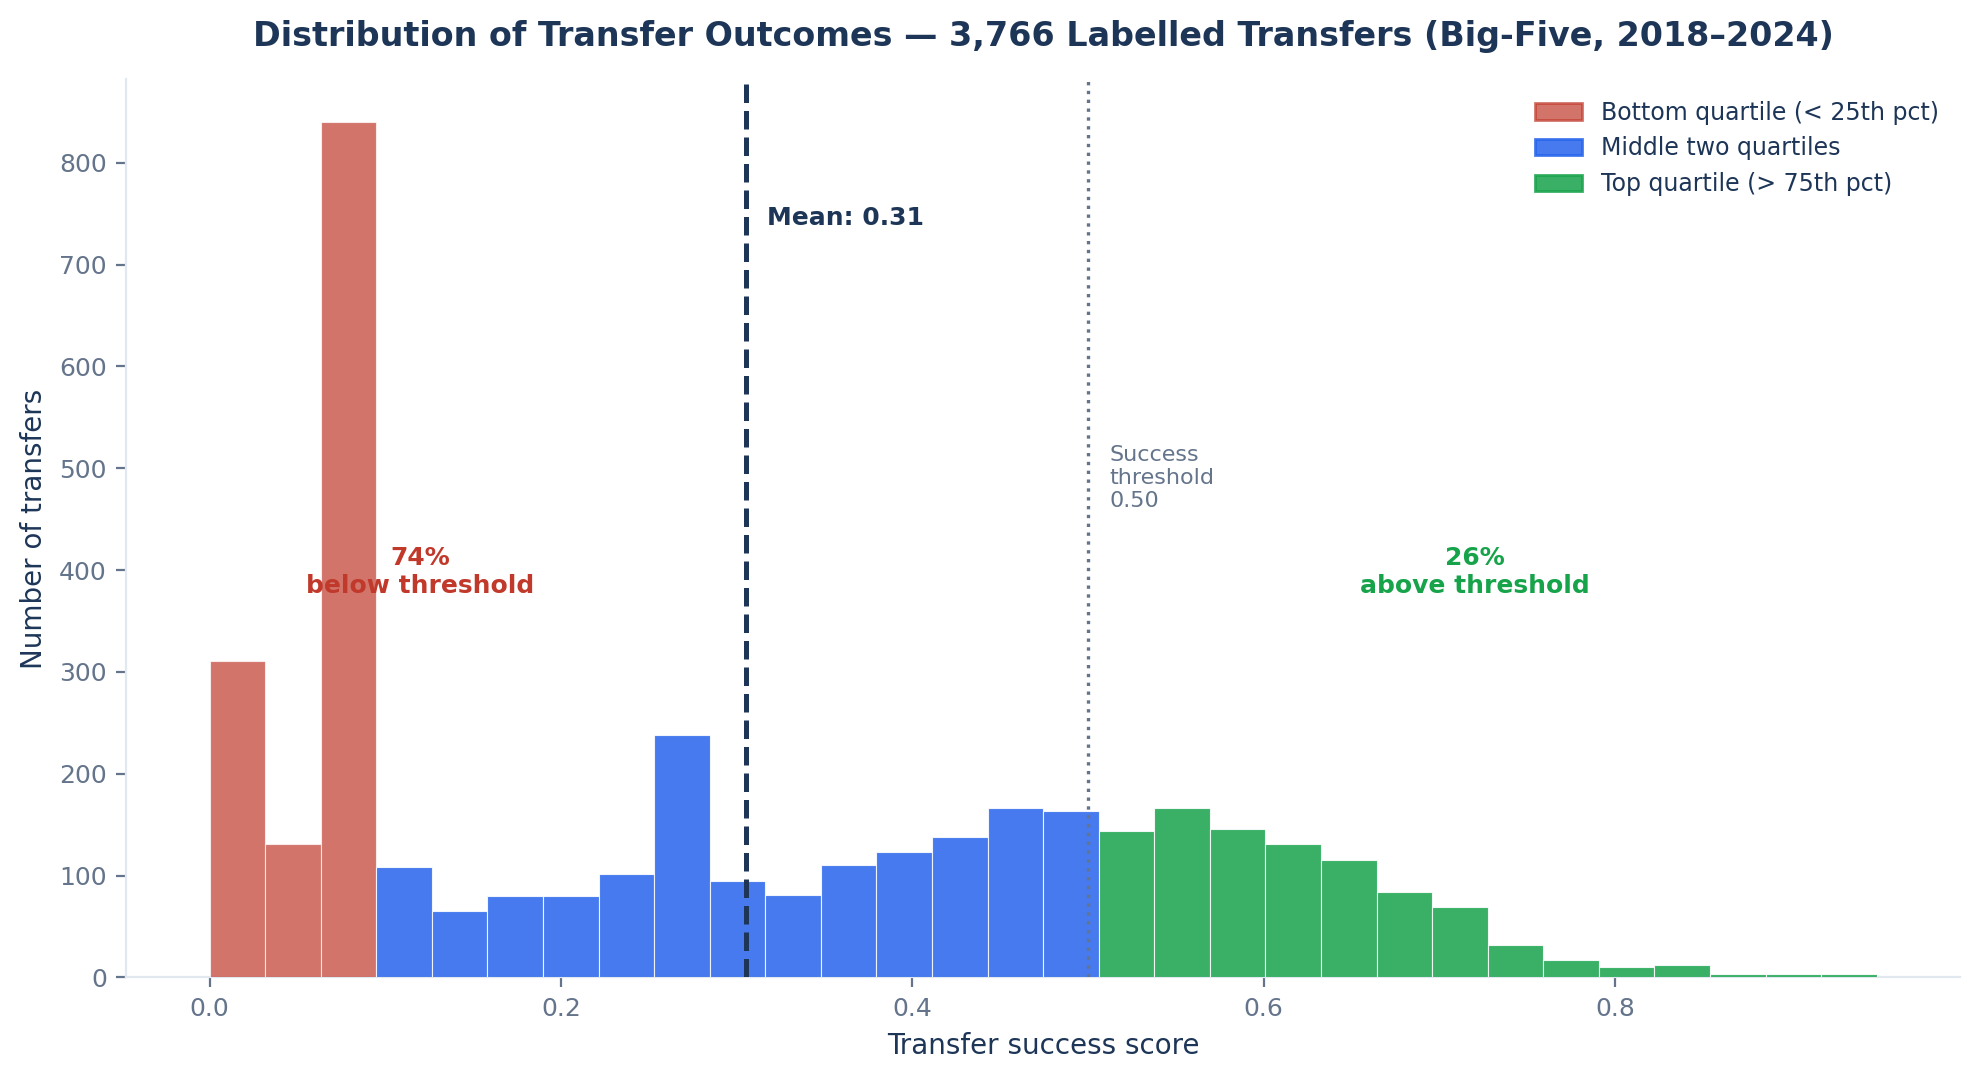
\includegraphics[width=\textwidth]{05_outcome_distribution.png}
\caption{Distribution of transfer success scores across 3,766 labelled transfers. Red bars: bottom quartile (below 25th percentile). Blue bars: middle two quartiles. Green bars: top quartile (above 75th percentile). The dashed vertical line marks the population mean (0.305). The dotted line marks the 0.50 threshold.}
\label{fig:outcome_dist}
\end{figure}

\section{The Fit Surprise Signal}
\label{sec:fit_surprise}

\subsection{Motivation}

The three primary success components (playing time, goal contribution, retention) measure outcomes but do not cleanly separate player quality from player--club fit. A player who plays 3,000 minutes in their first season may do so because they are genuinely elite, not because they specifically fit the club's system. Conversely, a player who plays only 1,200 minutes at a Champions League club may be systemically mismatched despite being excellent by any absolute standard.

We want a signal that answers the specific question: \textit{given what we know about this player's history, did they play more or fewer minutes than their history would predict?} A positive answer -- the player outperformed expectations -- is evidence of tactical fit. A negative answer is evidence of system mismatch, regardless of whether the player was objectively good or bad.

\subsection{Construction}

For each player at their new club in season $y1$, we define:

\begin{equation}
\label{eq:fit_surprise_raw}
\text{fit\_surprise\_raw}_i = m_{y1,i} - \hat{m}_{i}
\end{equation}

where $\hat{m}_{i}$ is the player's expected minutes share at the new club, estimated from their rolling two-season average appearance percentage at their previous club:

\begin{equation}
\hat{m}_{i} = \frac{1}{2} \sum_{k=1}^{2} \text{apps\_pct\_season}_{i, t-k}
\end{equation}

\subsection{Centering and normalisation}

The raw fit surprise signal has a population mean of approximately $-0.22$. This systematic negative offset reflects a structural feature of the transfer market: players who move clubs tend to move to clubs with higher competition for places, resulting in lower average playing time than their previous club. If we use the raw signal, the model would penalise quality upgrades -- exactly the opposite of the intended behaviour.

We correct this by centring on the \textbf{population median} rather than zero:

\begin{equation}
\label{eq:fit_surprise_centred}
\phi_{i}^{\text{raw}} = \text{fit\_surprise\_raw}_i - \tilde{\mu}
\end{equation}

where $\tilde{\mu}$ is the population median of \texttt{fit\_surprise\_raw} across all training transfers. This transforms the signal from ``did this player play more than their own previous season?'' to ``did this player play more than the typical player who made a similar type of transfer?'' -- a meaningful distinction.

The centred signal is clipped to $[-0.5, +0.5]$ and mapped to $[0, 1]$ to produce the final $\phi_i$:

\begin{equation}
\label{eq:fit_surprise_final}
\phi_i = \frac{\min(\max(\phi_{i}^{\text{raw}}, -0.5), +0.5) + 0.5}{1.0}
\end{equation}

Transfers for which a two-season baseline is not available (approximately 49\% of the training set) receive a neutral value of $\phi_i = 0.5$.

\subsection{Validation}

Figure~\ref{fig:fit_surprise} shows the relationship between fit surprise and transfer success score. The Spearman rank correlation is $\rho = 0.444$ -- the highest univariate correlation with success score of any feature in the dataset. Players in the top third of fit surprise (those who outperformed expectations most substantially) average a success score of 0.432, compared to 0.208 for players in the bottom third.

\begin{figure}[H]
\centering
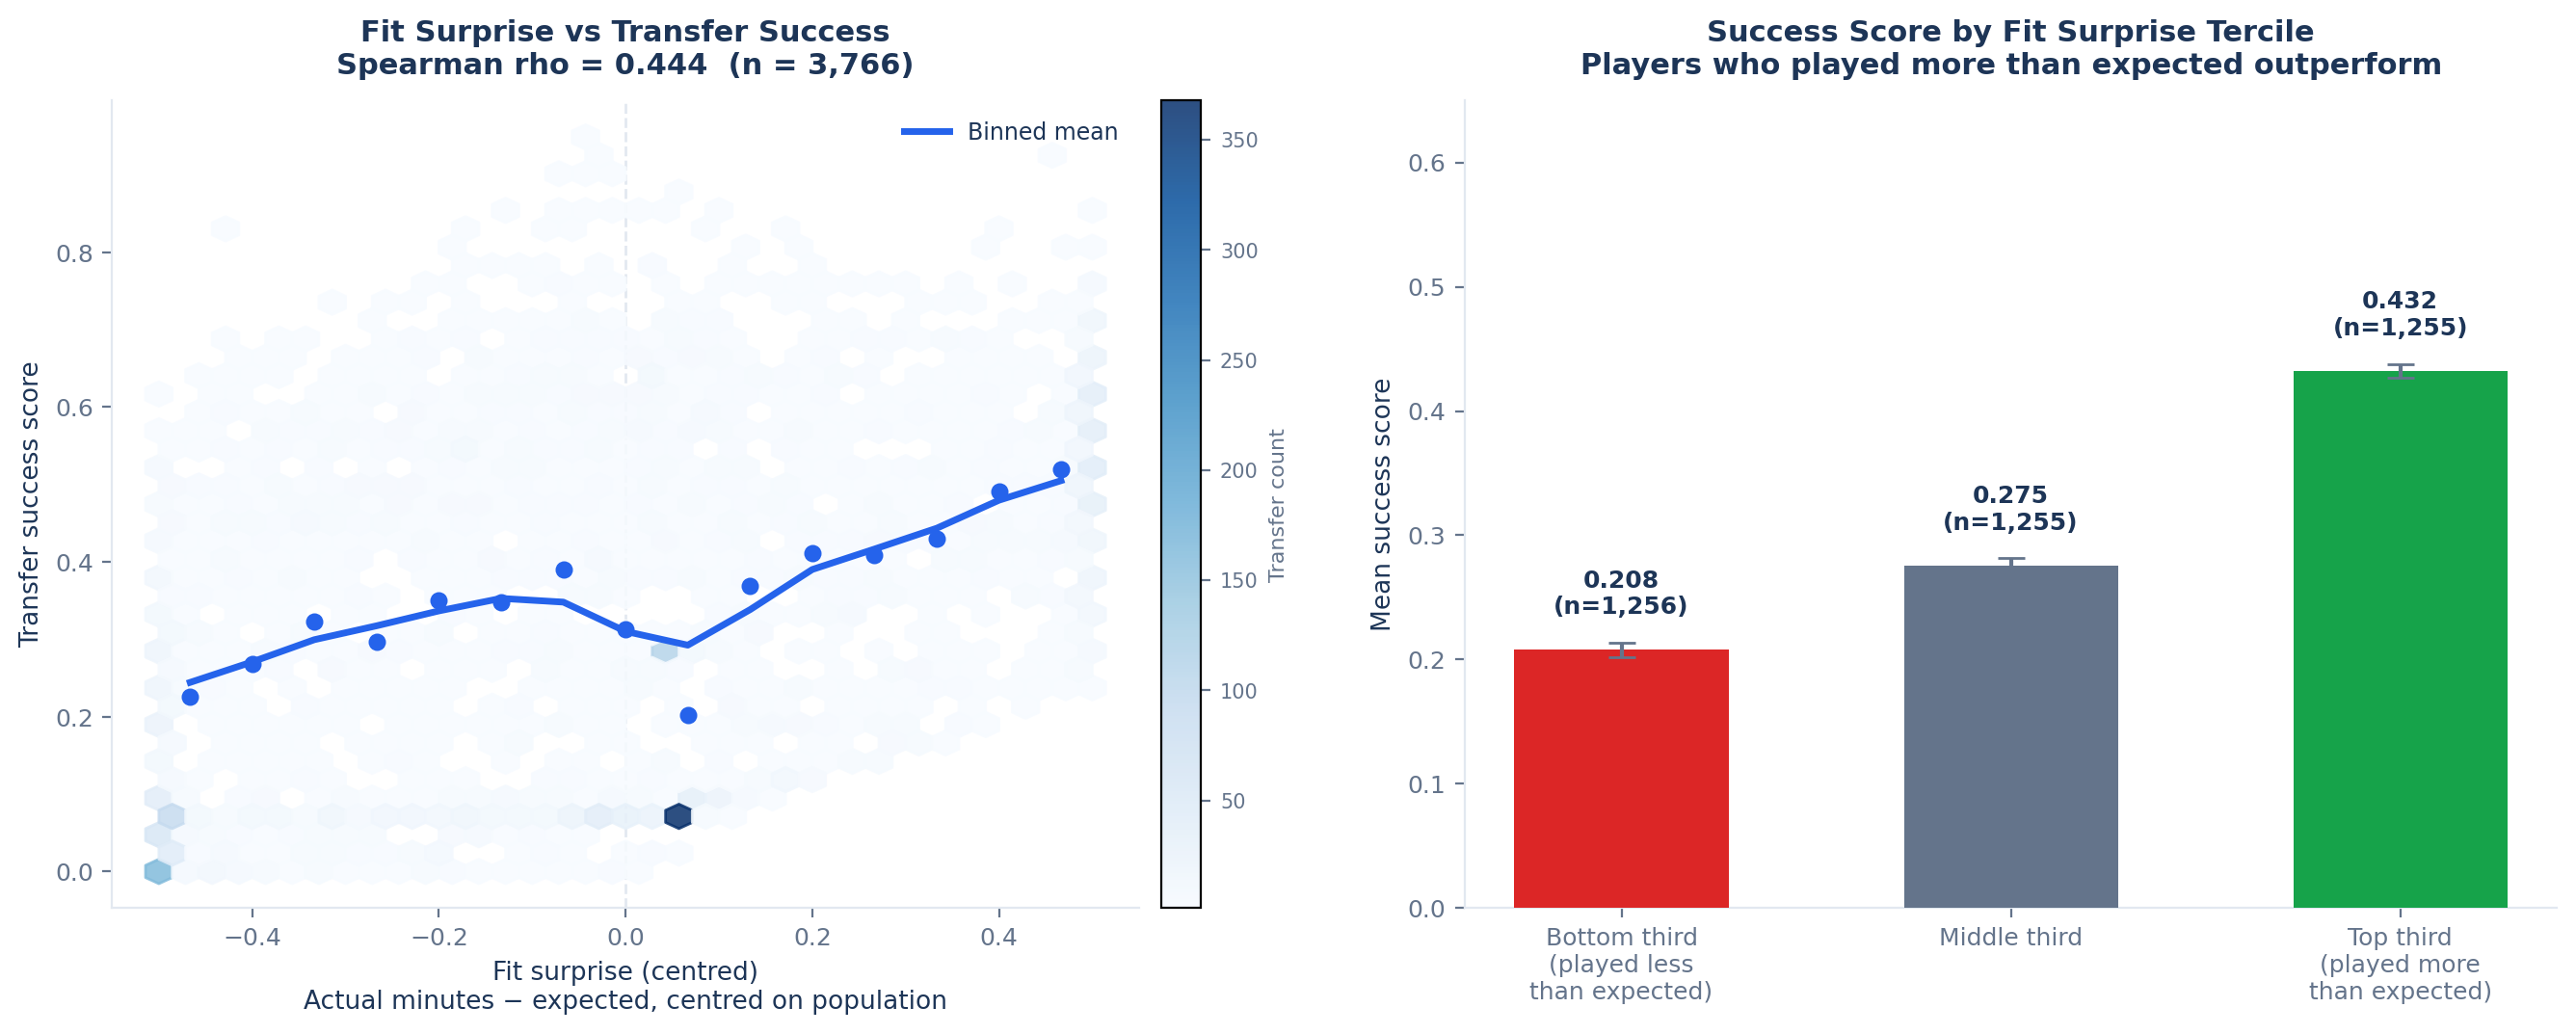
\includegraphics[width=\textwidth]{10_fit_surprise.png}
\caption{Left: Hexbin density plot of fit surprise versus transfer success score. The trend line shows a clear positive relationship ($\rho = 0.444$). Right: Mean success score by fit surprise tercile. Players in the top third (played more than expected given their history) achieve more than twice the mean success score of those in the bottom third.}
\label{fig:fit_surprise}
\end{figure}

\subsection{Impact on tactical differentiation}

Beyond its univariate correlation with success, fit surprise plays a critical structural role in producing tactically differentiated model outputs. Without the fit surprise component in the label, the model produces nearly identical recommendations for a high-press tactical profile (analogous to Liverpool under Klopp, PPDA $\approx 7.5$) and a low-block defensive profile (analogous to Mourinho-era sides, PPDA $\approx 14.0$): 13 of 15 candidates appear on both shortlists. With fit surprise included in the label, overlap falls to 2 of 15. The signal teaches the model that the same player will achieve different tactical outcomes in different systems.

% ══════════════════════════════════════════════════════════════════════════════
\chapter{Feature Engineering}
\label{chap:features}
% ══════════════════════════════════════════════════════════════════════════════

\section{Player Features}
\label{sec:player_features}

The player tower receives 15 input features. These are divided into four groups: performance statistics, physical/biographical proxies, injury indicators, and position encoding. All features are standardised (zero mean, unit variance) using scalers fitted on the training set.

\subsection{Performance statistics}

\begin{longtable}{p{3.5cm} p{9.5cm}}
\toprule
\textbf{Feature} & \textbf{Description and computation} \\
\midrule
\texttt{goals\_p90} & Goals scored per 90 minutes, from Transfermarkt appearances. Computed from the season preceding the transfer. \\[4pt]
\texttt{assists\_p90} & Assists per 90 minutes. Same source and window. \\[4pt]
\texttt{yellow\_cards\_p90} & Yellow cards per 90 minutes. Used as a proxy for defensive aggression and pressing intensity. Players who press hard and win the ball in opponent territory commit more fouls and receive more cards. \\[4pt]
\texttt{avg\_min\_per\_game} & Average minutes played per appearance in the preceding season. Distinguishes reliable starters (80+ minutes per appearance) from rotation players (45--55 minutes) from occasional substitutes (15--25 minutes). Encodes manager trust independently of appearance rate. \\[4pt]
\texttt{apps\_pct\_season} & Proportion of league matches in which the player appeared, in the preceding season. Separates persistent starters from players with interrupted seasons due to injury, suspension, or tactical choices. \\[4pt]
\texttt{npxg\_p90} & Non-penalty expected goals per 90. For the current dataset, proxied as \texttt{goals\_p90} $\times$ 0.88, reflecting the typical relationship between goals and non-penalty xG across Big Five players. This is a heuristic: true npxG requires event-level shot data (see Chapter~\ref{chap:limitations}). \\[4pt]
\texttt{key\_passes\_p90} & Key passes (passes leading directly to a shot) per 90. Proxied as \texttt{assists\_p90} $\times$ 2.0, reflecting the approximate ratio of key passes to recorded assists in event data. Again heuristic; the true value requires FBref passing table data, which is unavailable via static scraping. \\[4pt]
\texttt{mv\_momentum\_12m} & Relative market value change over the preceding 12 months: $(\text{MV}_{t} - \text{MV}_{t-12}) / \text{MV}_{t-12}$. Captures whether the player is perceived as improving, stable, or declining. A rising market value reflects a player in form or development; a declining value may signal that the player is past their peak or recovering from a serious injury. \\
\bottomrule
\caption{Player performance features.}
\label{tab:player_perf_features}
\end{longtable}

\subsection{Injury indicators}

\begin{table}[H]
\centering
\caption{Player injury features.}
\label{tab:injury_features}
\begin{tabular}{p{3.5cm} p{9.5cm}}
\toprule
\textbf{Feature} & \textbf{Description} \\
\midrule
\texttt{injury\_days\_last\_2y} & Total days missed to injury in the 24 months preceding the transfer. Scraped from Transfermarkt's individual injury pages. Directly predicts first-season playing time availability. Population mean: 17.4 days; 8.8\% of players have at least one serious injury in the window. \\[4pt]
\texttt{has\_serious\_injury} & Binary. 1 if any single injury in the prior three years exceeded 60 days (an approximate threshold for structural injuries including ACL and Achilles ruptures). Captures long-term risk that aggregate days missed may understate. \\
\bottomrule
\end{tabular}
\end{table}

\subsection{Market value and position}

\begin{table}[H]
\centering
\caption{Market value and position features.}
\label{tab:mv_pos_features}
\begin{tabular}{p{3.5cm} p{9.5cm}}
\toprule
\textbf{Feature} & \textbf{Description} \\
\midrule
\texttt{log\_value} & Natural logarithm of market value in millions EUR. Log transformation applied because the market value distribution is right-skewed (range: approximately 0.1M to 200M EUR). Serves as a quality proxy that the model uses to calibrate output expectations against competition level. \\[4pt]
\texttt{pos\_ATT}, \texttt{pos\_DEF}, \texttt{pos\_MID}, \texttt{pos\_GK} & One-hot encoding of position group. Allows the player tower to learn position-specific latent representations. A goalkeeper and a striker cannot be compared on the same statistical scale; the one-hot encoding creates separate regions of the embedding space for each position. \\
\bottomrule
\end{tabular}
\end{table}

\section{Excluded Player Features and Rationale}
\label{sec:excluded_features}

Several intuitively appealing features were considered and explicitly excluded. The rationale for each exclusion is documented here, as these decisions are as important as the decisions about what to include.

\textbf{Transfer age.} Transfer age was included in early model iterations and produced a Spearman correlation of $+0.72$ between age and fit score at inference time, effectively sorting recommendations by age. Age is a legitimate predictor of transfer success in aggregate (younger players have more adaptation time and longer development windows), but in the scouting context it is better handled as a hard filter applied by the user before the model runs. Including it in the model produced outputs that a scout would experience as an age-sorted list with cosmetic variation, not a fit-sorted list.

\textbf{League of origin one-hot.} Including the player's previous league as a one-hot encoding baked in a 10-point Premier League premium that was independent of player quality: a Premier League attacker with identical statistics to a Ligue 1 attacker was scored systematically higher, biasing recommendations against continental signings. The destination league is already represented in the club tower via league one-hot encoding.

\textbf{Tackles won, interceptions per 90.} These are available from FBref's miscellaneous statistics table and are genuine tactical signals, particularly for pressing intensity. They were excluded because FBref coverage is 47\% in training and 64\% in the scouting pool -- a material train/inference coverage mismatch. A model that learns these features on a biased 47\% subsample of training data may learn the signal but also learn selection effects (which types of players have FBref data), producing biased inference on the 36\% of the scouting pool that lacks FBref data. The features appear in the application UI for display purposes but do not enter the neural network.

\textbf{Progressive passes, progressive carries, pass completion, take-ons.} These FBref passing and possession features are blocked by JavaScript rendering (see Section~\ref{chap:data}). They are proxied in the UI from position-age-value lookup tables but do not enter the model.

\textbf{Contract months remaining at time of transfer.} This variable is only available in its current state on Transfermarkt, not historically. Using current contract data for historical training rows would introduce temporal leakage.

\section{Club Features}
\label{sec:club_features}

The club tower receives 9 input features: 4 tactical metrics and a 5-league one-hot encoding.

\subsection{Tactical metrics}

The four tactical metrics are derived from football-data.co.uk per-match data, aggregated by club-season. They are proxies for the true tactical metrics that would be available from event-level tracking data.

\begin{table}[H]
\centering
\caption{Club tactical features and their derivation.}
\label{tab:club_features}
\begin{tabular}{p{3cm} p{5.5cm} p{5cm}}
\toprule
\textbf{Feature} & \textbf{Formula} & \textbf{Interpretation} \\
\midrule
\texttt{possession\_pct} & $\frac{\text{shots\_for}}{\text{shots\_for} + \text{shots\_against}} \times 100$ & Shot share as a proxy for possession. Correlates approximately $r = 0.85$ with Opta tracked possession data. \\[6pt]
\texttt{ppda} & $20 - \text{fouls\_per\_game} \times 0.45$ & Proxy for pressing intensity. High-press clubs commit more fouls high up the pitch, resulting in lower proxy PPDA. True PPDA (passes allowed per defensive action in the opponent's half) requires event-level data. \\[6pt]
\texttt{directness\_idx} & $\frac{\text{shots\_on\_target}}{\text{shots\_total}}$ & Shot quality ratio. Possession-based teams take more speculative long shots, producing a lower ratio. Counter-attacking teams generate fewer but higher-quality chances. \\[6pt]
\texttt{line\_height\_m} & Derived from corners\_against per game, mapped to $[25, 65]$ metres & Teams defending deep concede more corners as opponents pin them back. Higher corners against $\Rightarrow$ lower defensive line. \\
\bottomrule
\end{tabular}
\end{table}

Figure~\ref{fig:tactical_map} shows the distribution of all 150 clubs in the possession--PPDA tactical space.

\begin{figure}[H]
\centering
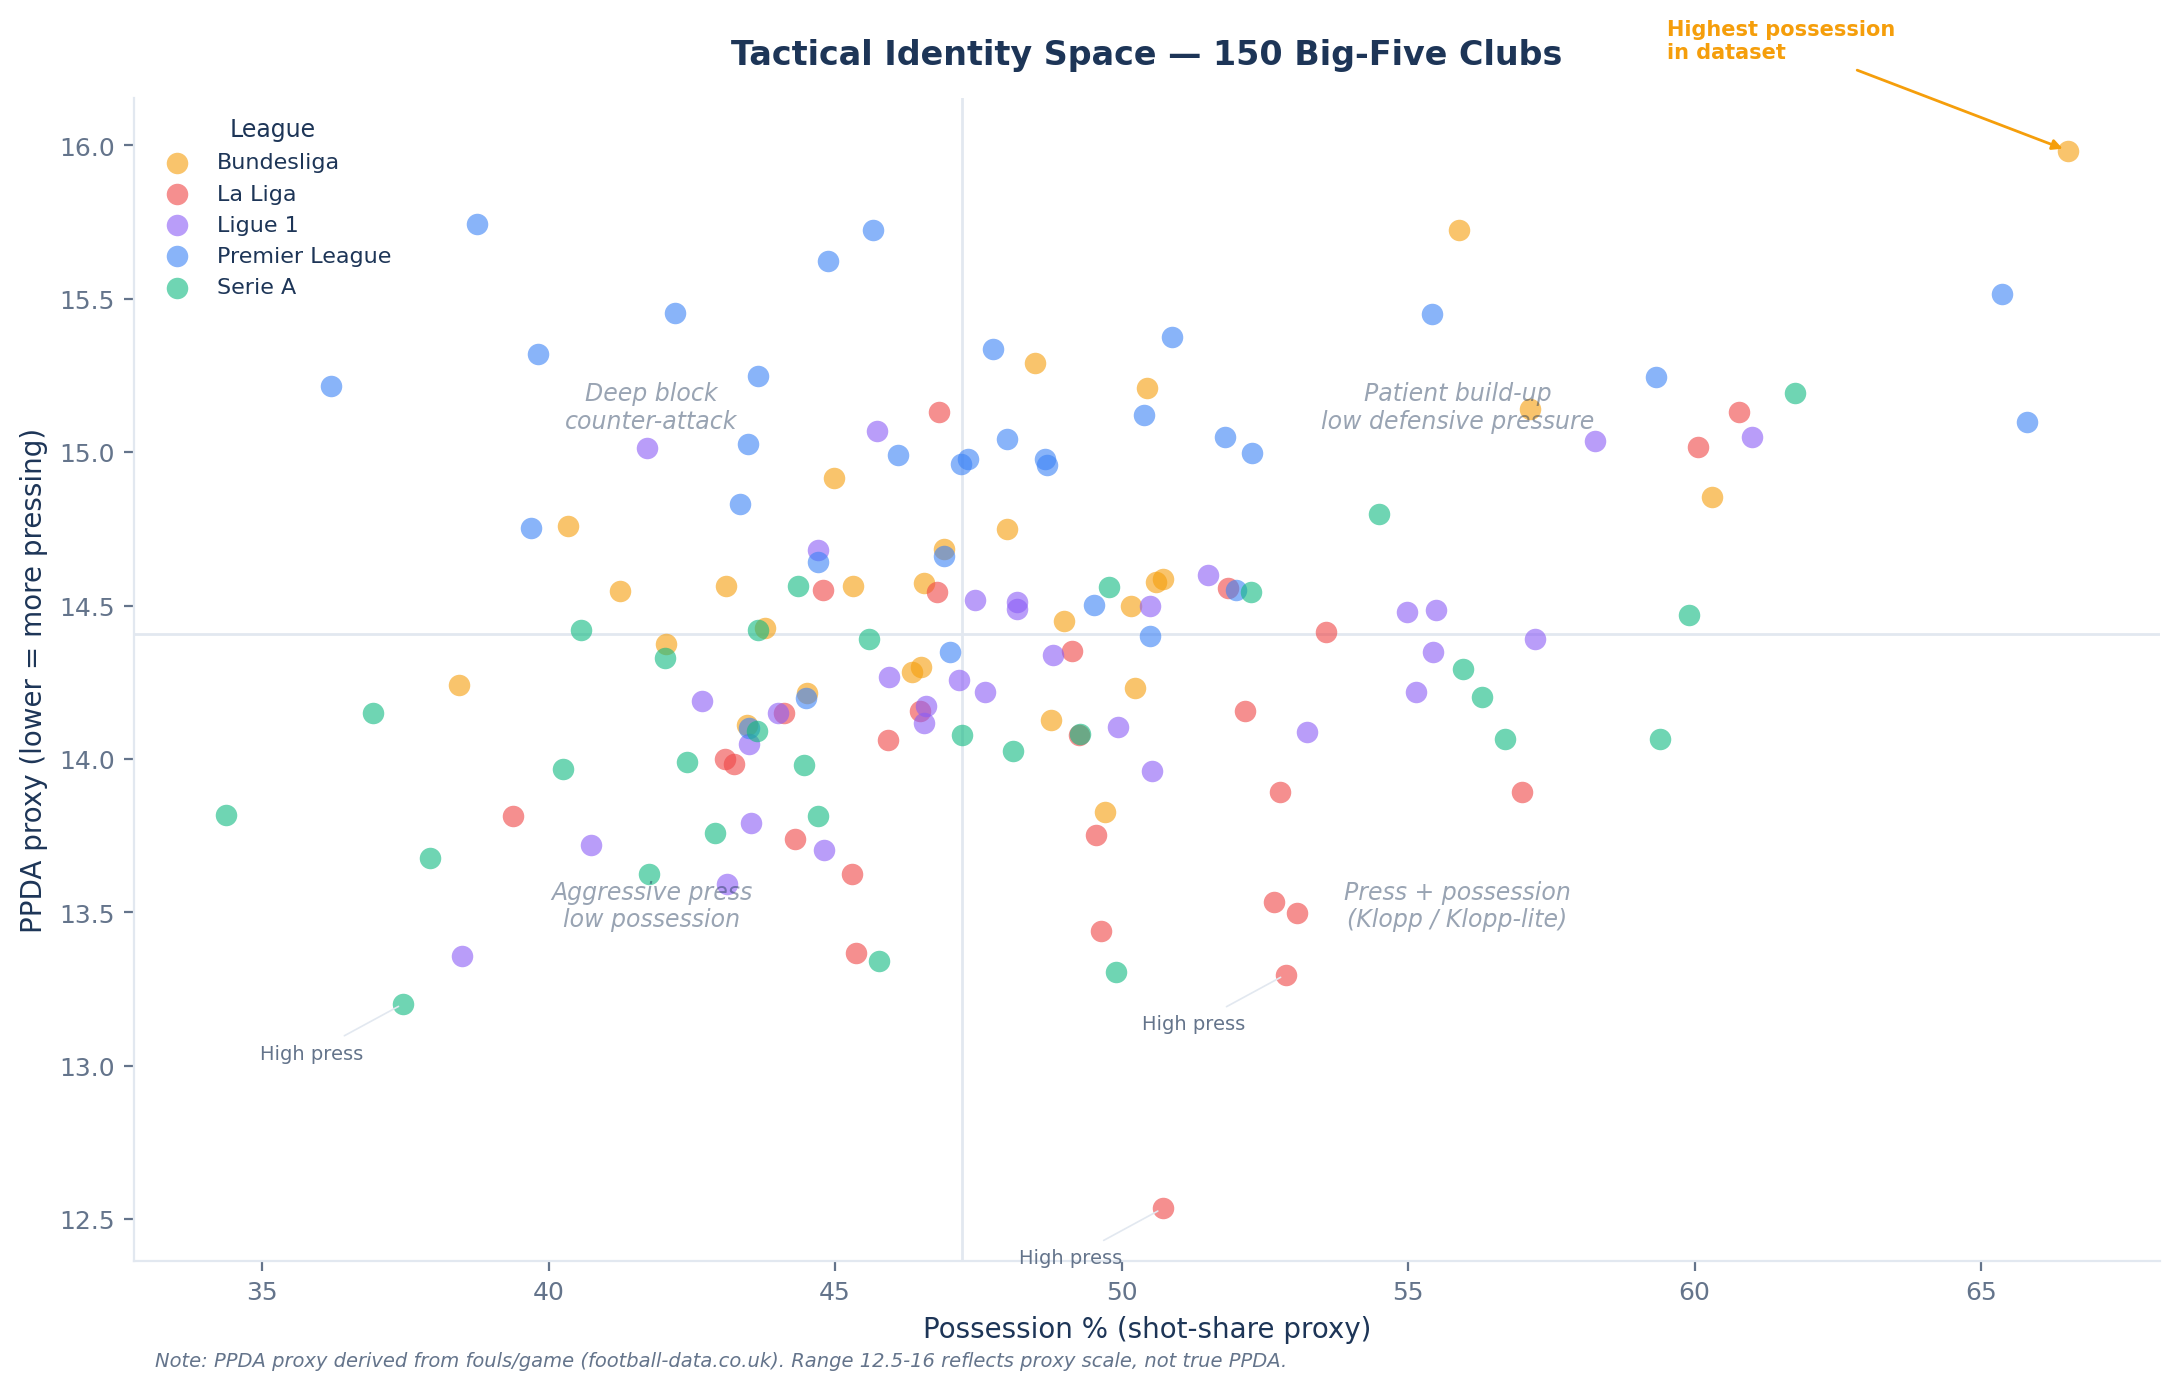
\includegraphics[width=\textwidth]{04_tactical_map.png}
\caption{Tactical identity of 150 Big-Five clubs in the possession--pressing space. Each point represents one club-season pair. League membership is colour-coded. Lower PPDA indicates more pressing intensity. The quadrant labels indicate the stylistic archetype associated with each region of the tactical space.}
\label{fig:tactical_map}
\end{figure}

\subsection{League encoding}

A 5-class one-hot encoding of the destination league (Premier League, La Liga, Bundesliga, Serie A, Ligue 1) is included in the club tower. This allows the model to learn league-specific dynamics in the club representation without encoding league origin in the player representation (which would create the Premier League premium bias described in Section~\ref{sec:excluded_features}).

\section{Transfer Context}

A single transfer context feature enters the head MLP directly (not through either tower):

\begin{table}[H]
\centering
\begin{tabular}{p{3cm} p{10cm}}
\toprule
\textbf{Feature} & \textbf{Description} \\
\midrule
\texttt{log(fee\_eur\_m)} & Natural log of transfer fee in millions EUR. Enters the head as a scalar, not through either tower, because it is a property of the specific transfer transaction rather than a property of either the player or the club in isolation. \\
\bottomrule
\end{tabular}
\end{table}

% ══════════════════════════════════════════════════════════════════════════════
\chapter{Model Architecture}
\label{chap:model}
% ══════════════════════════════════════════════════════════════════════════════

\section{Design Rationale}

The fundamental modelling question is: given a player profile $\mathbf{p}$ and a club tactical profile $\mathbf{c}$, predict the expected success score $\hat{y}$ of the transfer.

The simplest approach is a standard MLP that takes a concatenated vector $[\mathbf{p}; \mathbf{c}; \text{ctx}]$ as input. The problem with concatenation is that the model can only learn fixed-weight linear combinations of player and club features. It cannot learn that ``player pressing intensity'' and ``club pressing demand'' are interacting dimensions in the same latent space -- that a player with high pressing intensity benefits specifically from a club with high pressing demand, and is penalised specifically by a club that prefers passive defence.

The two-tower architecture addresses this by learning separate latent representations for the player and the club, then modelling their interaction explicitly. The interaction is implemented via the Hadamard product (element-wise multiplication) and absolute difference of the two embeddings:

\begin{equation}
\text{interaction} = [\mathbf{e}_p \odot \mathbf{e}_c \; ; \; |\mathbf{e}_p - \mathbf{e}_c|]
\end{equation}

The Hadamard product captures alignment: if player embedding dimension $k$ is high (the player excels on that latent dimension) and club embedding dimension $k$ is also high (the club demands strength on that dimension), the product is high -- signalling compatibility. The absolute difference captures mismatch: if the player and club diverge on dimension $k$, the difference is large regardless of sign.

\section{Network Architecture}

\subsection{Player tower}

\begin{equation}
\label{eq:player_tower}
\mathbf{e}_p = f_p(\mathbf{x}_p) : \mathbb{R}^{15} \to \mathbb{R}^{32}
\end{equation}

\begin{align*}
\mathbf{h}_1^p &= \text{GELU}(\mathbf{W}_1^p \mathbf{x}_p + \mathbf{b}_1^p), \quad \mathbf{W}_1^p \in \mathbb{R}^{64 \times 15} \\
\mathbf{h}_1^p &\leftarrow \text{Dropout}(\mathbf{h}_1^p, p=0.15) \\
\mathbf{e}_p    &= \mathbf{W}_2^p \mathbf{h}_1^p + \mathbf{b}_2^p, \quad \mathbf{W}_2^p \in \mathbb{R}^{32 \times 64}
\end{align*}

\subsection{Club tower}

\begin{equation}
\label{eq:club_tower}
\mathbf{e}_c = f_c(\mathbf{x}_c) : \mathbb{R}^{9} \to \mathbb{R}^{32}
\end{equation}

\begin{align*}
\mathbf{h}_1^c &= \text{GELU}(\mathbf{W}_1^c \mathbf{x}_c + \mathbf{b}_1^c), \quad \mathbf{W}_1^c \in \mathbb{R}^{32 \times 9} \\
\mathbf{h}_1^c &\leftarrow \text{Dropout}(\mathbf{h}_1^c, p=0.15) \\
\mathbf{e}_c    &= \mathbf{W}_2^c \mathbf{h}_1^c + \mathbf{b}_2^c, \quad \mathbf{W}_2^c \in \mathbb{R}^{32 \times 32}
\end{align*}

\subsection{Head MLP}

The head receives the concatenation of the Hadamard interaction, absolute difference, and transfer context:

\begin{equation}
\mathbf{z} = [\mathbf{e}_p \odot \mathbf{e}_c \; ; \; |\mathbf{e}_p - \mathbf{e}_c| \; ; \; \text{ctx}] \in \mathbb{R}^{65}
\end{equation}

\begin{align*}
\mathbf{h}_1^z &= \text{GELU}(\mathbf{W}_1^z \mathbf{z} + \mathbf{b}_1^z), \quad \mathbf{W}_1^z \in \mathbb{R}^{64 \times 65} \\
\mathbf{h}_1^z &\leftarrow \text{Dropout}(\mathbf{h}_1^z, p=0.15) \\
\mathbf{h}_2^z &= \text{GELU}(\mathbf{W}_2^z \mathbf{h}_1^z + \mathbf{b}_2^z), \quad \mathbf{W}_2^z \in \mathbb{R}^{64 \times 64} \\
\mathbf{h}_2^z &\leftarrow \text{Dropout}(\mathbf{h}_2^z, p=0.15) \\
\hat{y}        &= \sigma(\mathbf{w}_3^z \cdot \mathbf{h}_2^z + b_3^z)
\end{align*}

where $\sigma$ is the sigmoid function, constraining the output to $(0, 1)$.

The total parameter count is approximately 15,000 to 20,000. This is deliberately modest given the training set size of approximately 2,636 samples. Scaling the model would increase overfitting risk faster than it would improve generalisation on this dataset.

Figure~\ref{fig:architecture} provides a visual summary of the complete architecture.

\begin{figure}[H]
\centering
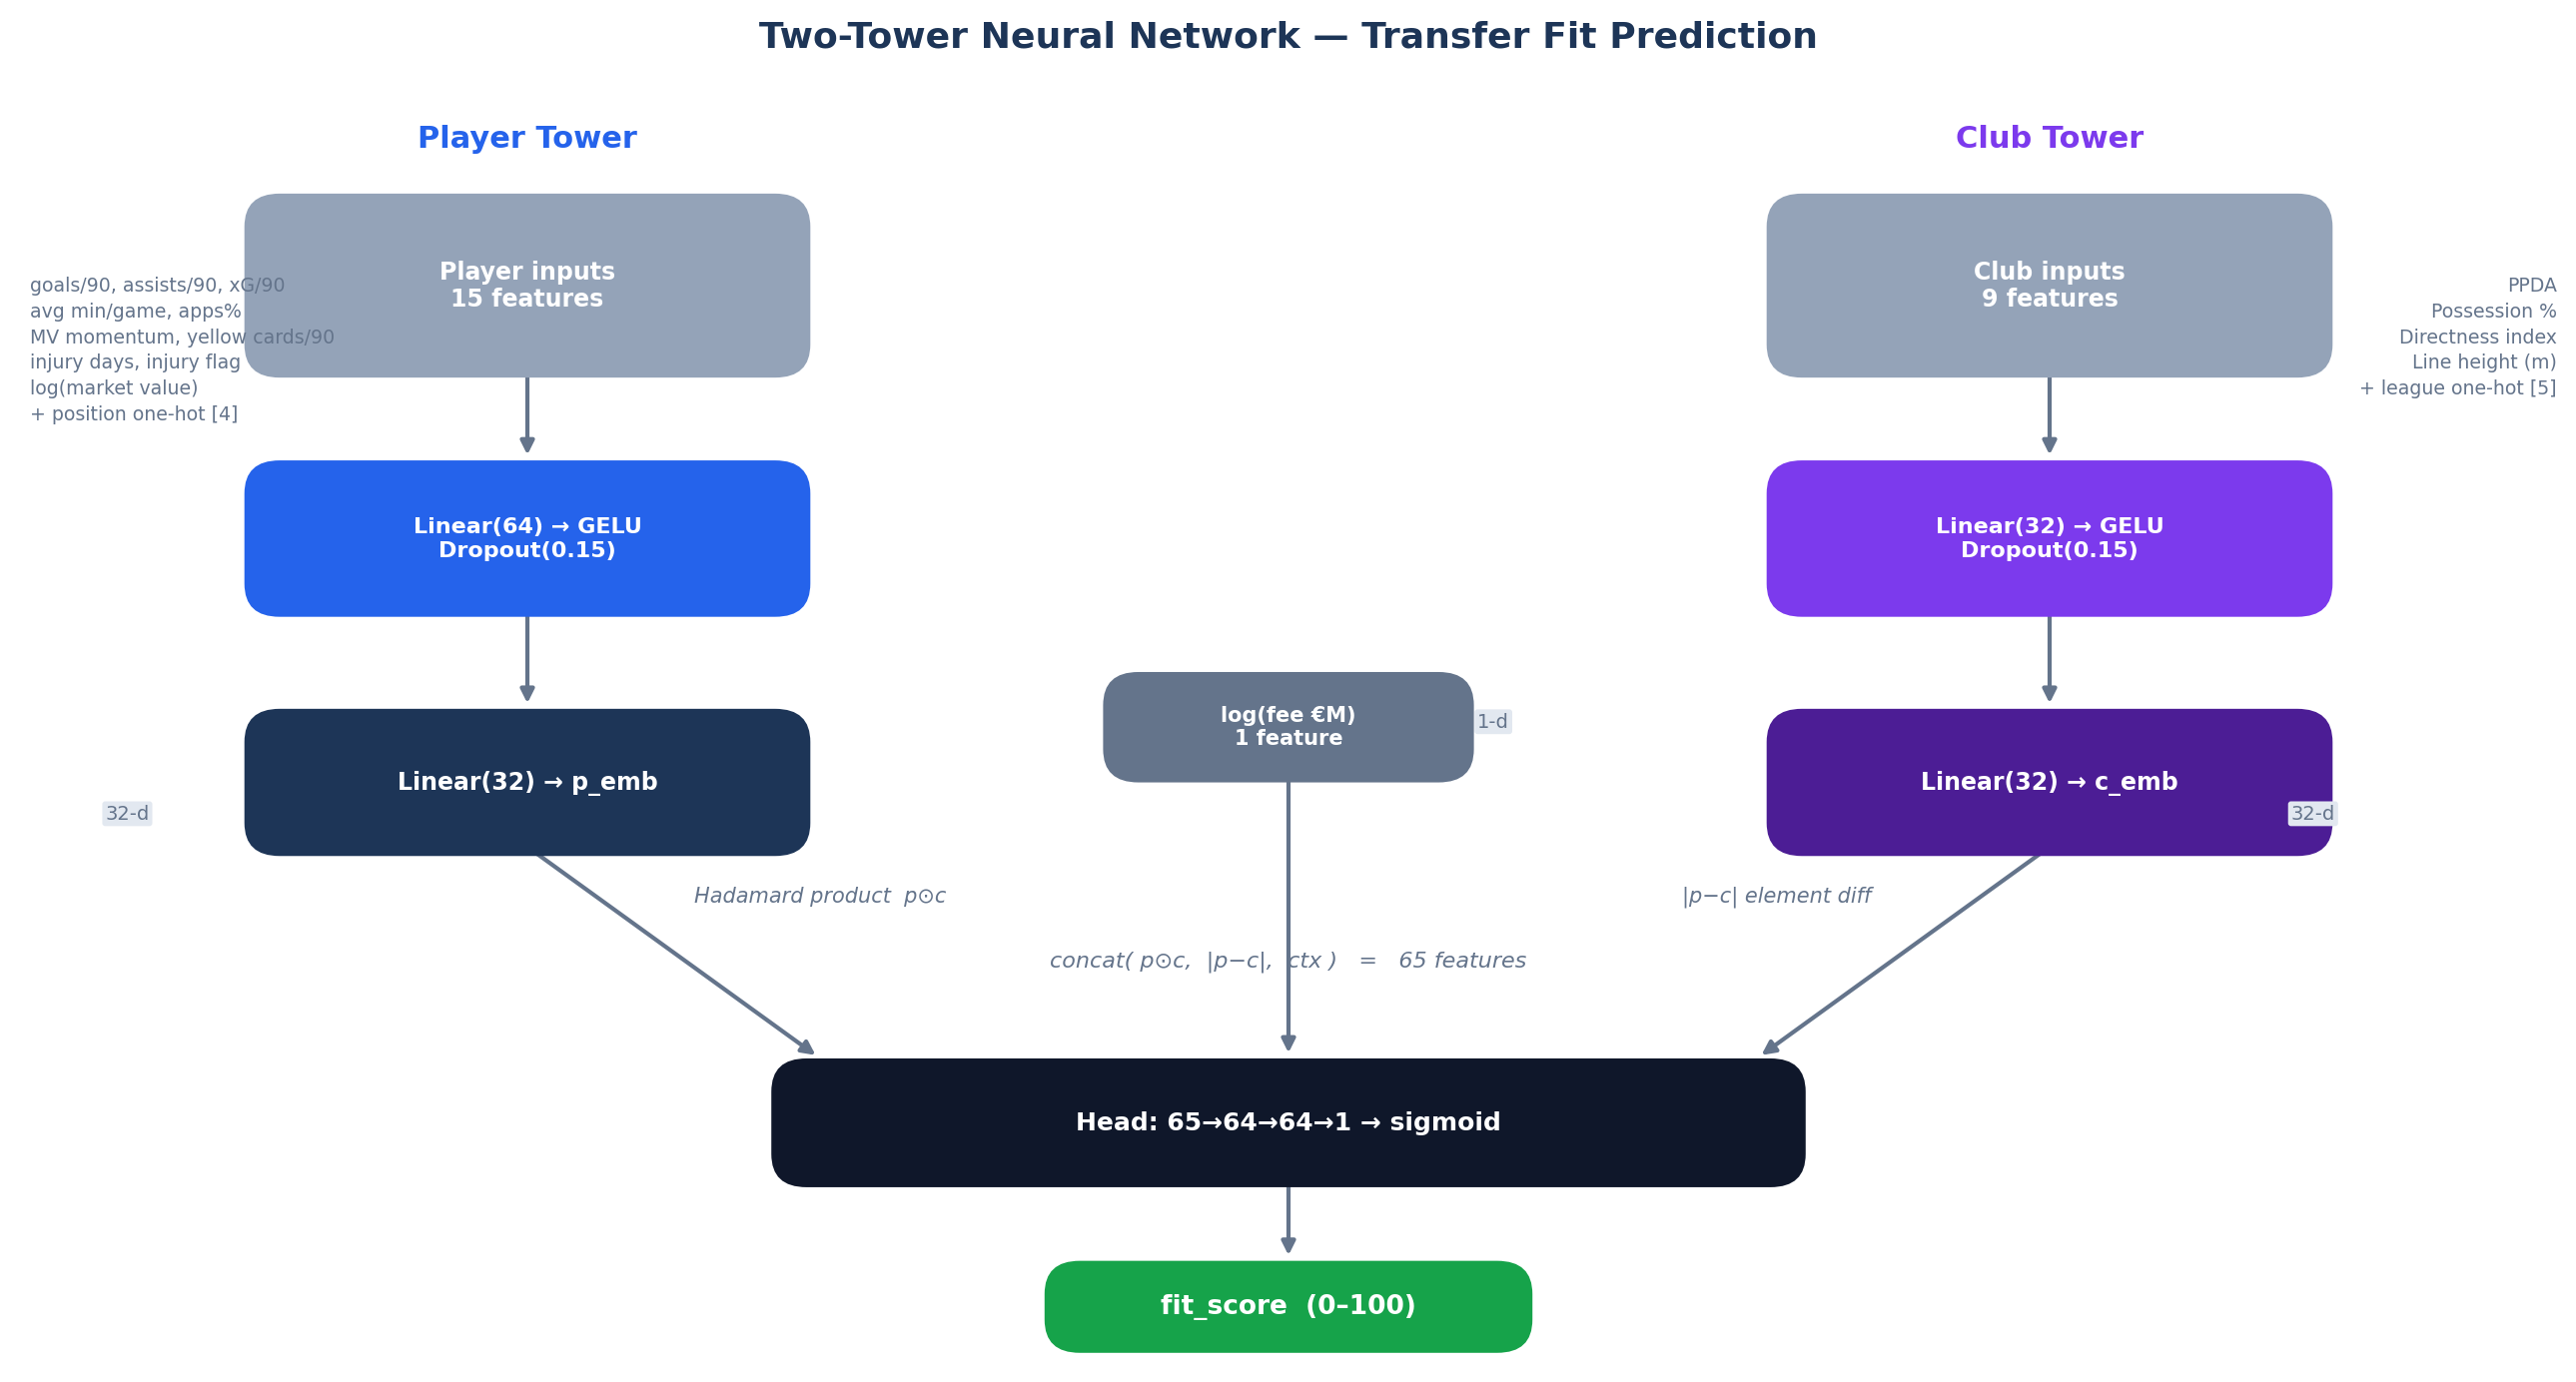
\includegraphics[width=\textwidth]{01_architecture.png}
\caption{Two-tower architecture. The player tower (left, blue) maps 15 player features to a 32-dimensional embedding. The club tower (right, purple) maps 9 club features to a parallel 32-dimensional embedding. The head MLP receives the Hadamard product, absolute difference, and transfer context as input and outputs a predicted success score in $[0, 1]$.}
\label{fig:architecture}
\end{figure}

\section{Training Protocol}

\begin{table}[H]
\centering
\caption{Training hyperparameters.}
\label{tab:training}
\begin{tabular}{ll}
\toprule
\textbf{Hyperparameter} & \textbf{Value} \\
\midrule
Loss function       & Mean squared error (MSE) \\
Optimiser           & Adam \\
Learning rate       & $5 \times 10^{-4}$ \\
Weight decay        & $1 \times 10^{-4}$ \\
Batch size          & 256 \\
Max epochs          & 300 \\
Early stopping      & Patience 25, monitoring validation MSE \\
LR scheduler        & ReduceLROnPlateau, factor 0.5, patience 10, min $10^{-5}$ \\
Dropout             & 0.15 at all layers \\
Activation          & GELU \\
\bottomrule
\end{tabular}
\end{table}

Early stopping typically fires around epoch 120 to 180. The best validation MSE achieved is 0.0430. MSE is used as the training objective because it is a well-understood regression loss and the success score is continuous. The operational metric (Spearman rank correlation) is evaluated post-hoc on the test set.

% ══════════════════════════════════════════════════════════════════════════════
\chapter{Results and Analysis}
\label{chap:results}
% ══════════════════════════════════════════════════════════════════════════════

\section{Baseline Comparisons}

Table~\ref{tab:benchmarks} presents the performance of the two-tower model against three baselines on the held-out test set.

\begin{table}[H]
\centering
\caption{Model performance on held-out test set (approximately 565 transfers, entirely unseen players). Best values in \textbf{bold}.}
\label{tab:benchmarks}
\begin{tabular}{lrrr}
\toprule
\textbf{Model} & \textbf{R$^2$} & \textbf{Spearman $\rho$} & \textbf{MAE} \\
\midrule
Cosine similarity baseline & 0.0001 & 0.008 & 0.173 \\
Gradient Boosted Machine   & 0.088  & 0.325 & 0.167 \\
Linear regression          & \textbf{0.127}  & 0.353 & \textbf{0.160} \\
\textbf{Two-tower (ours)}  & 0.122  & \textbf{0.370} & \textbf{0.160} \\
\bottomrule
\end{tabular}
\end{table}

\subsection{Interpreting R$^2$ = 0.122}

An R$^2$ of 0.122 -- explaining 12.2\% of variance in transfer success -- may appear low. In the context of this problem, it is not. Transfer success is driven substantially by variables that no external dataset captures: manager tenure during the player's first season (a manager who signed the player may be sacked before the player can prove themselves), dressing room dynamics, the player's personal circumstances at the time of the move, and timing of injuries relative to the adaptation period. A model trained on public data explaining 12\% of variance in a genuinely noisy target is a material signal, not a noise artefact.

The cosine similarity baseline -- which scores players purely on how similar their statistics are to the club's current squad average -- achieves $\rho = 0.008$, essentially random. This establishes that the label is not trivially predictable and that the model is learning genuine signal.

\subsection{Spearman correlation as the operational metric}

Spearman rank correlation ($\rho$) is the operationally relevant metric in this context. A scout does not require a precise probability estimate; they require a ranking that puts the right players at the top. At $\rho = 0.370$, the two-tower model's ranking is substantially better than chance ($\rho = 0$) and better than the GBM baseline ($\rho = 0.325$, $\Delta = +4.5$ percentage points).

The two-tower does not outperform linear regression on R$^2$. This is expected: linear regression has a structural advantage on small datasets with near-Gaussian residuals. The two-tower's advantage is architectural -- the bilinear interaction between player and club embeddings captures non-linear compatibility effects that the linear model cannot represent. As the transfer database grows year over year, this structural advantage should compound while the linear model's performance ceiling remains fixed.

\section{Feature Importance}

Figure~\ref{fig:feature_importance} shows permutation importance for all 15 player features. Permutation importance is computed by shuffling each feature column independently across five random seeds, measuring the average drop in Spearman correlation, and reporting the mean.

\begin{figure}[H]
\centering
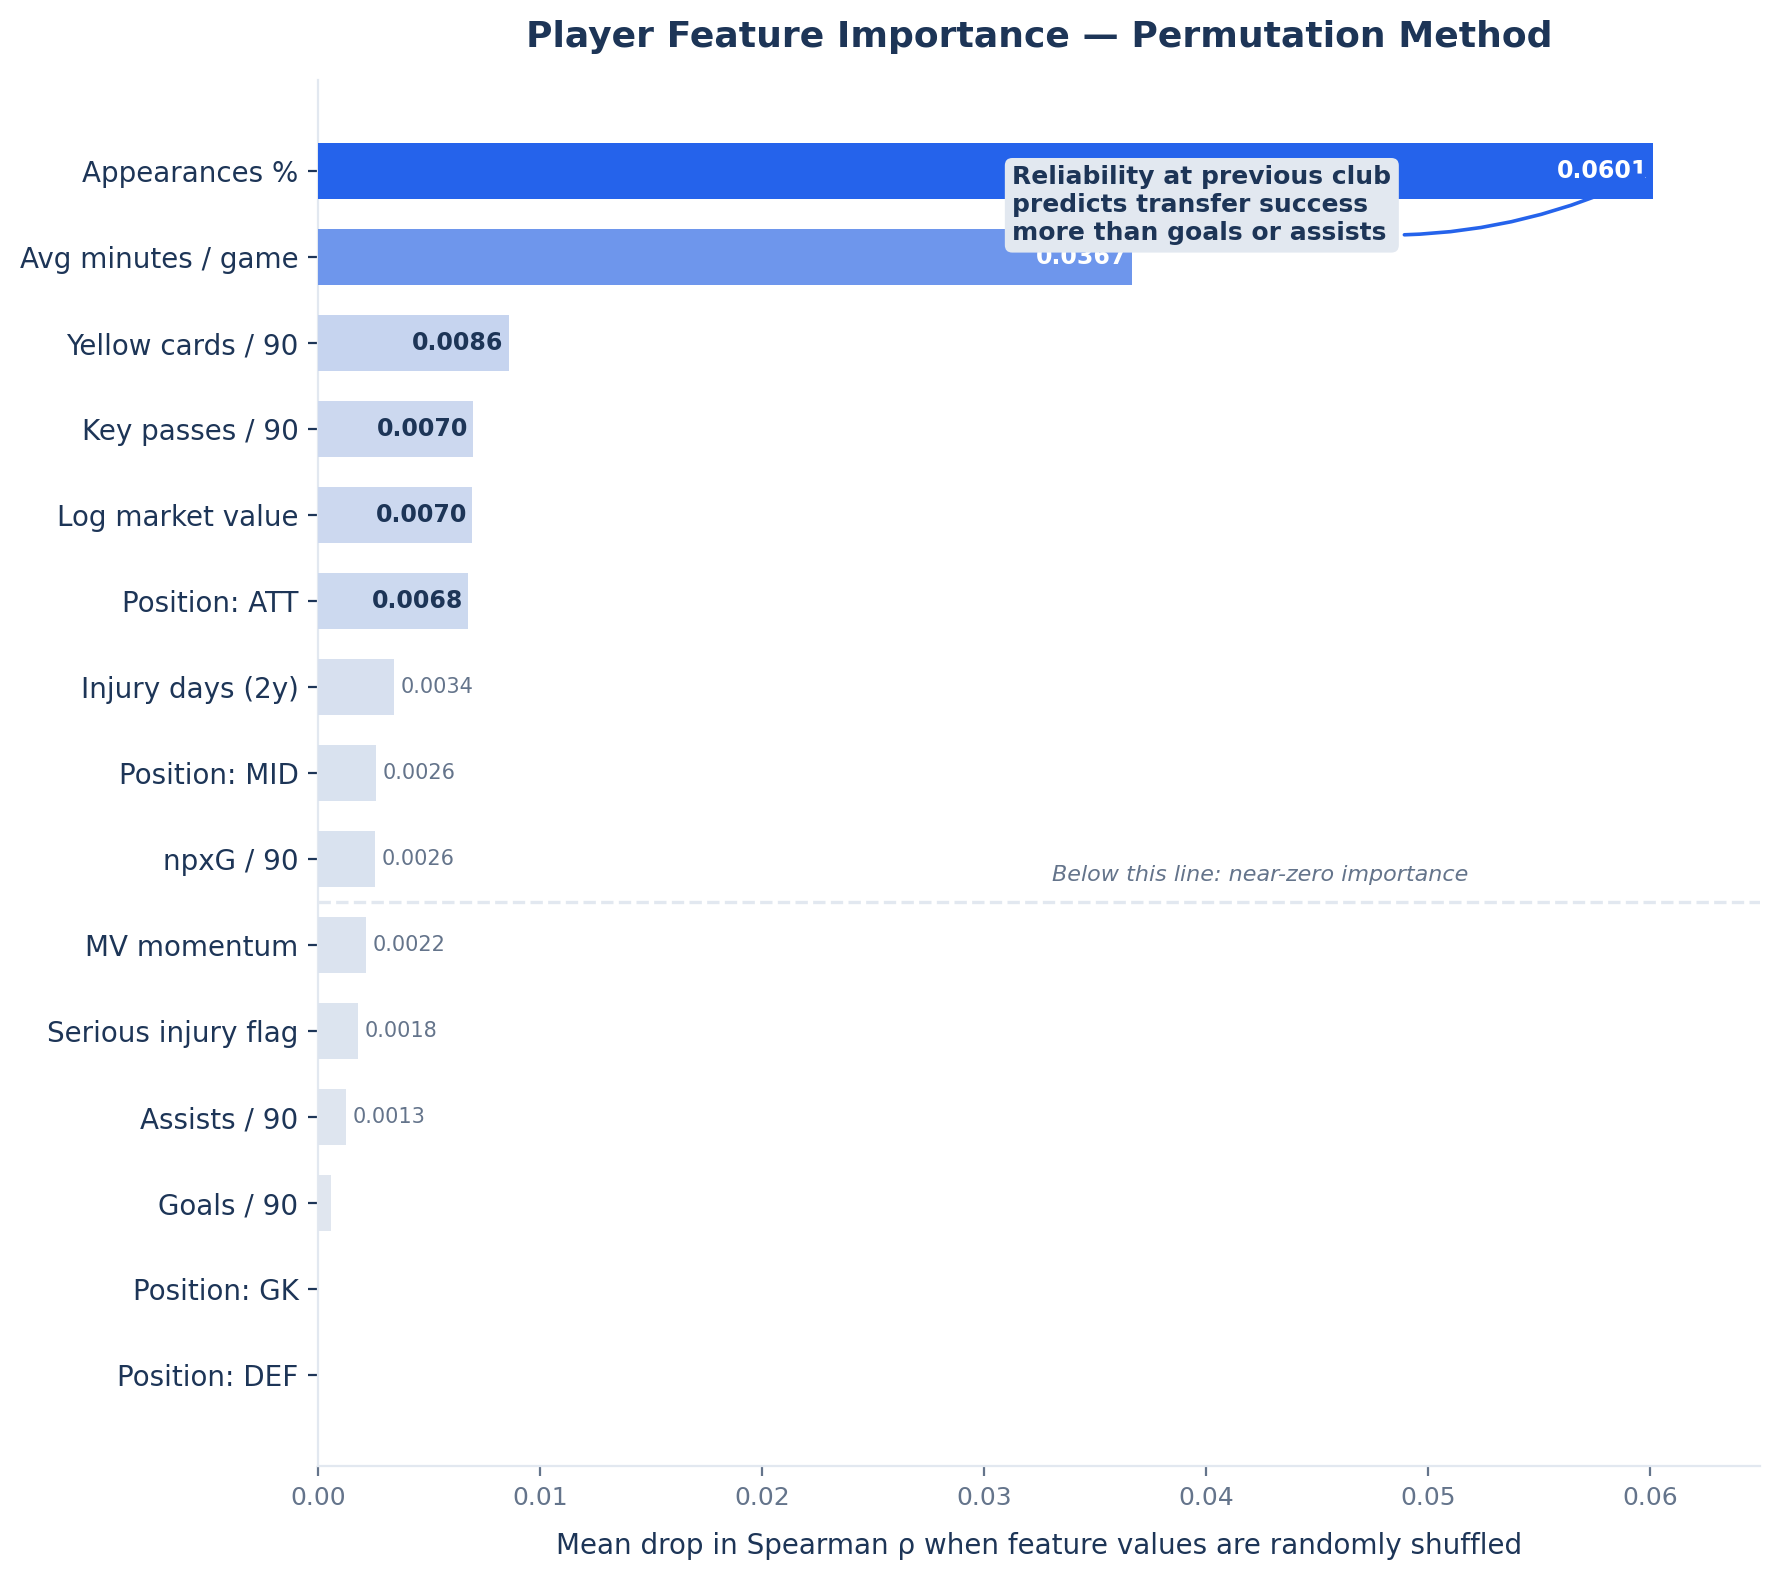
\includegraphics[width=\textwidth]{07_feature_importance.png}
\caption{Permutation feature importance for the trained two-tower model. Each bar represents the mean drop in Spearman rho on the training set when that feature's values are randomly permuted. Features highlighted in blue produce a drop exceeding 0.01; features in light grey produce negligible impact.}
\label{fig:feature_importance}
\end{figure}

The most striking finding is the dominance of availability metrics: \texttt{apps\_pct\_season} (importance 0.060) and \texttt{avg\_min\_per\_game} (0.037) together account for the vast majority of the model's explainable signal. \texttt{goals\_p90} and \texttt{assists\_p90} have importance near zero. This is a counterintuitive result with a straightforward explanation: whether a player \textit{played} at their previous club is a stronger predictor of whether they will \textit{play} at their new club than how many goals they scored when they did play. The model has learned that manager trust -- as revealed by playing time -- is the most transferable signal in the data.

The injury features (\texttt{injury\_days\_last\_2y}, \texttt{has\_serious\_injury}) show modest but non-zero importance. This is partly because their impact on the label is mediated by playing time (injured players play fewer minutes), meaning the playing time features already capture some of the injury signal.

\section{Embedding Space Analysis}

Figure~\ref{fig:embeddings} shows a t-SNE projection of the 32-dimensional player embeddings for all 2,700 players in the current scouting pool.

\begin{figure}[H]
\centering
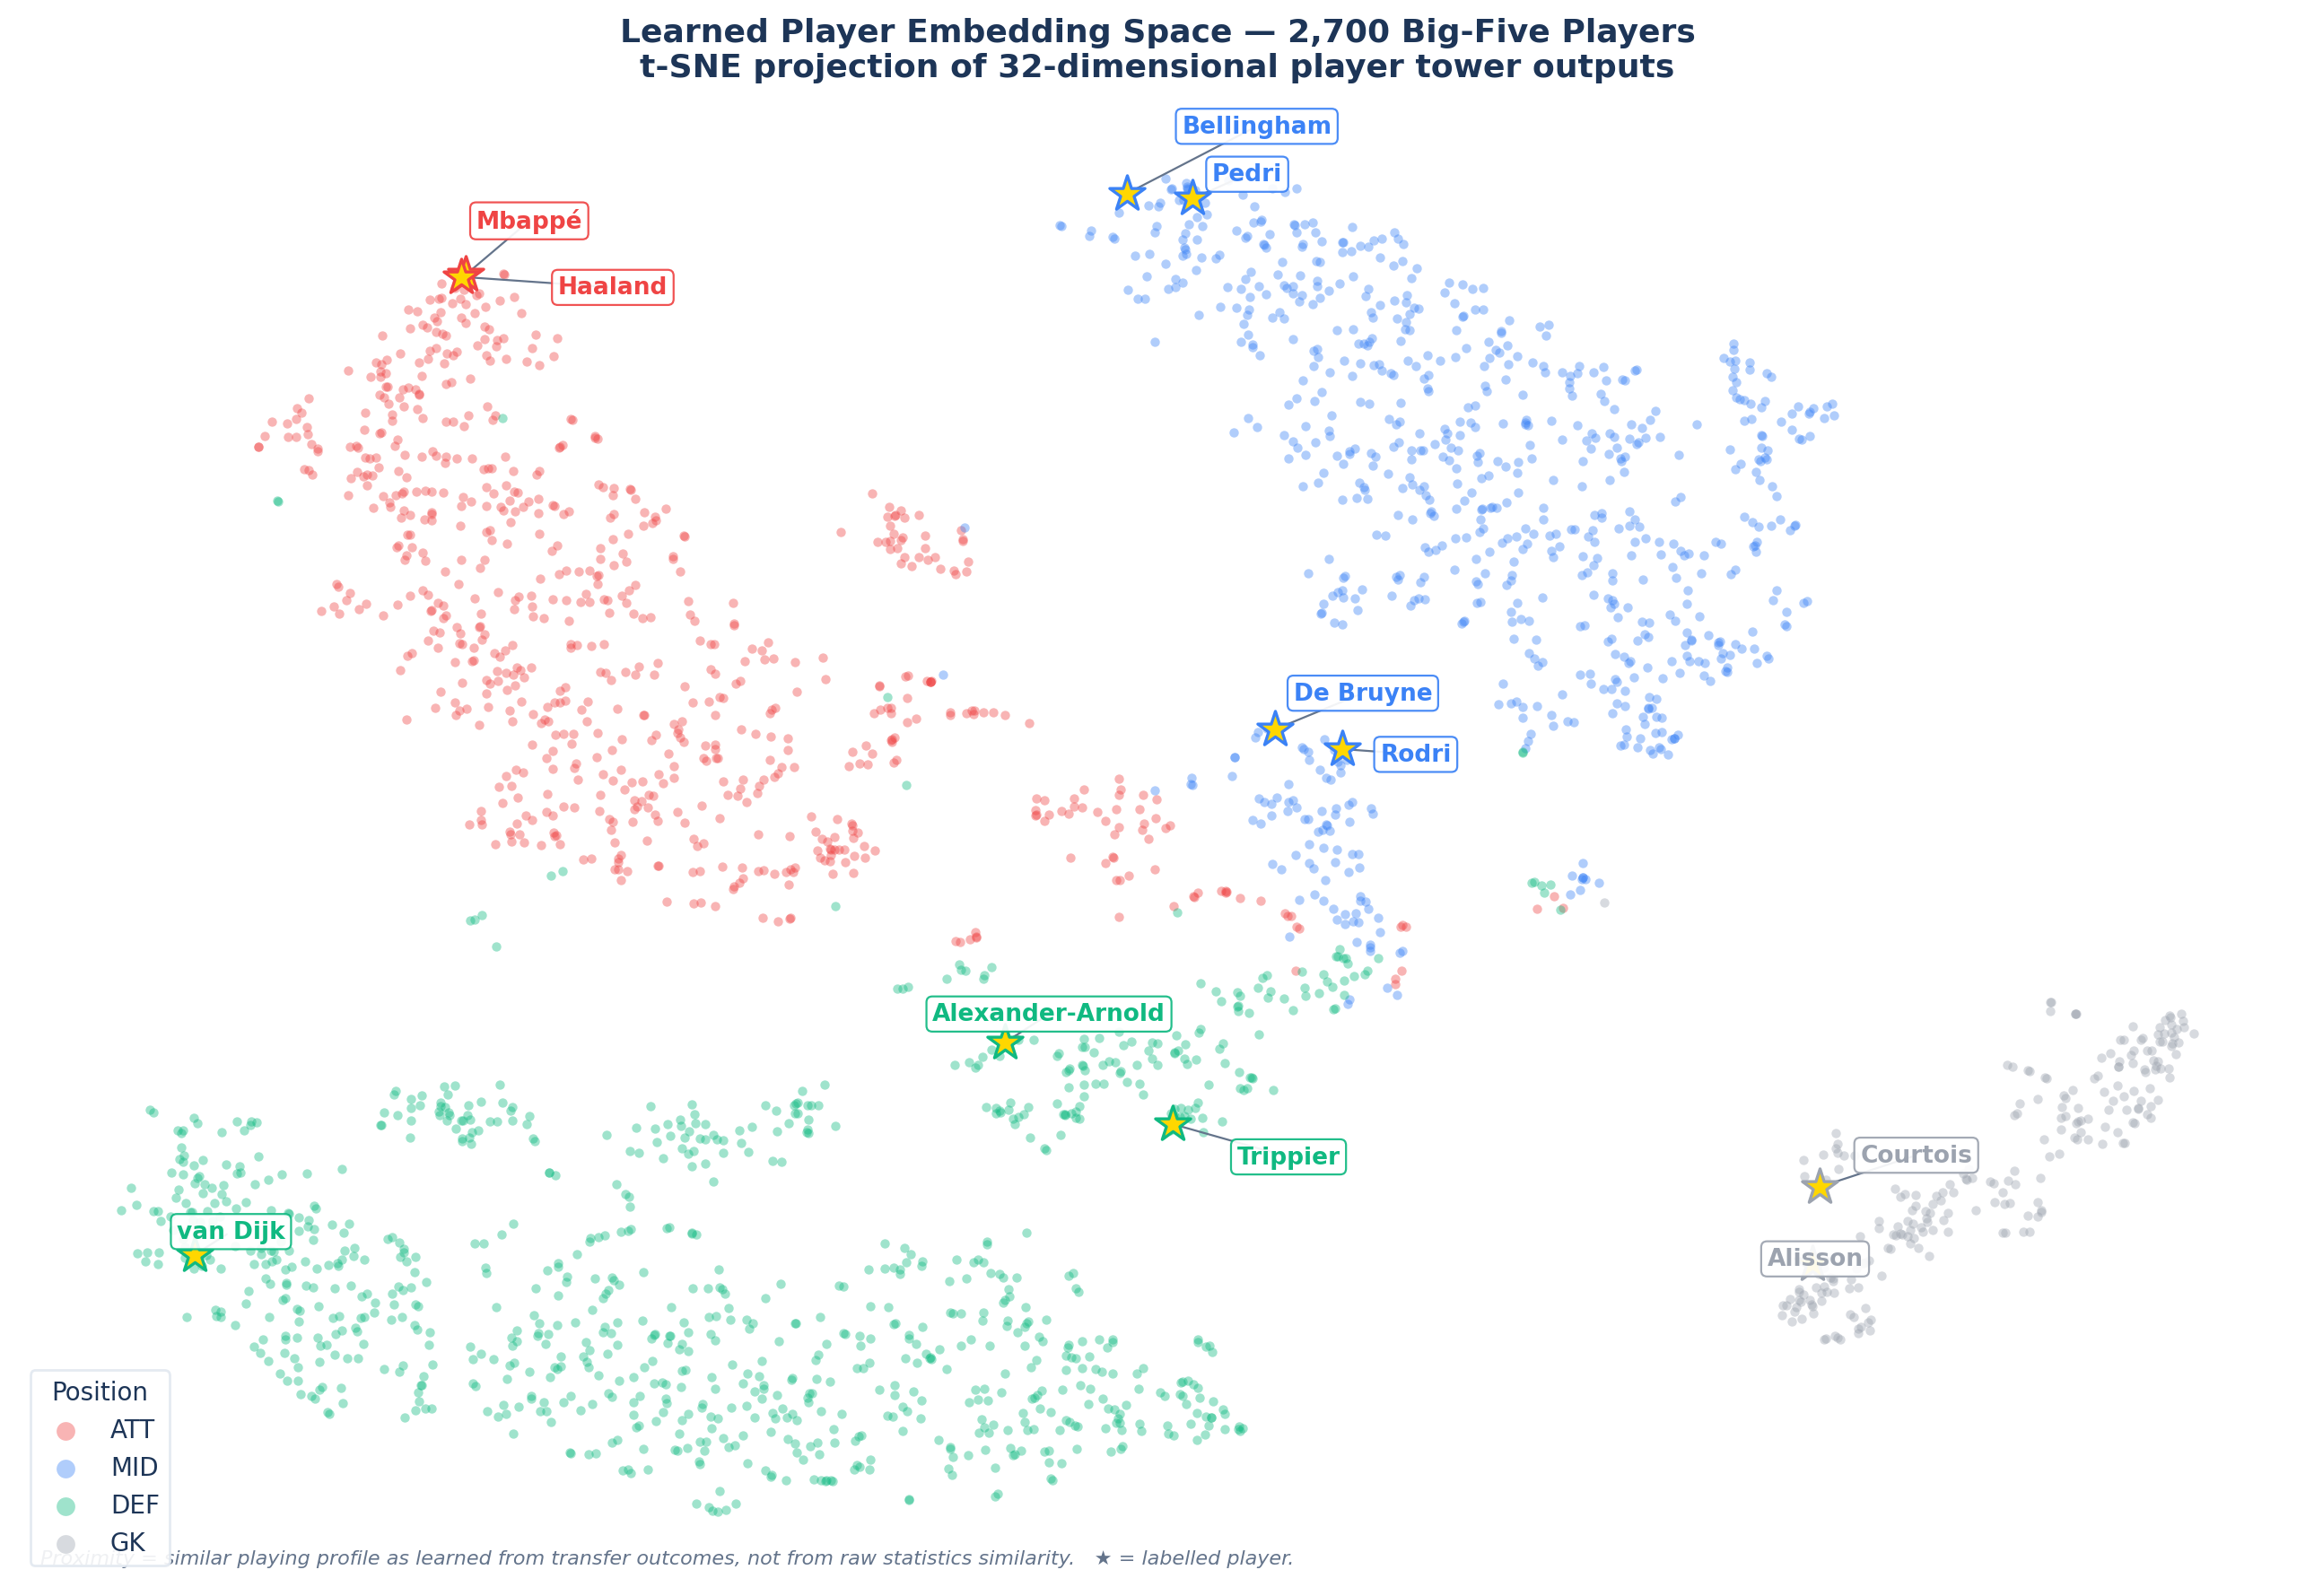
\includegraphics[width=\textwidth]{08_embedding_space.png}
\caption{t-SNE projection of 32-dimensional player tower embeddings for 2,700 Big-Five players (2024--25 season). Colours indicate position. Position was not included in the club tower and no explicit positional clustering loss was used. The model learned to separate positions from transfer outcomes alone.}
\label{fig:embeddings}
\end{figure}

Several observations are notable. First, the four positions separate cleanly despite position never appearing in the club tower and no explicit positional objective being used in training. The model discovered that attackers, midfielders, defenders, and goalkeepers succeed and fail at different clubs in systematically different ways, and encoded this in the embedding geometry. Second, within each position cluster, there is variation along continuous axes that likely correspond to stylistic dimensions (e.g., pressing intensity, technical orientation, physical versus technical profile) that the model has learned to separate from historical transfer outcomes. Third, the GK cluster is isolated and compact, consistent with the fact that goalkeepers are essentially incomparable to outfield players on most performance metrics.

The embedding space is a secondary product of training with operational value: it enables the ``Similar Players'' feature in the scouting application. Two players close in embedding space have similar playing profiles as revealed by where they succeeded and failed across all training transfers -- not merely similar raw statistics.

\section{Label Component Independence}

Figure~\ref{fig:label_corr} shows the Spearman rank correlation matrix between all four success score components and the composite label.

\begin{figure}[H]
\centering
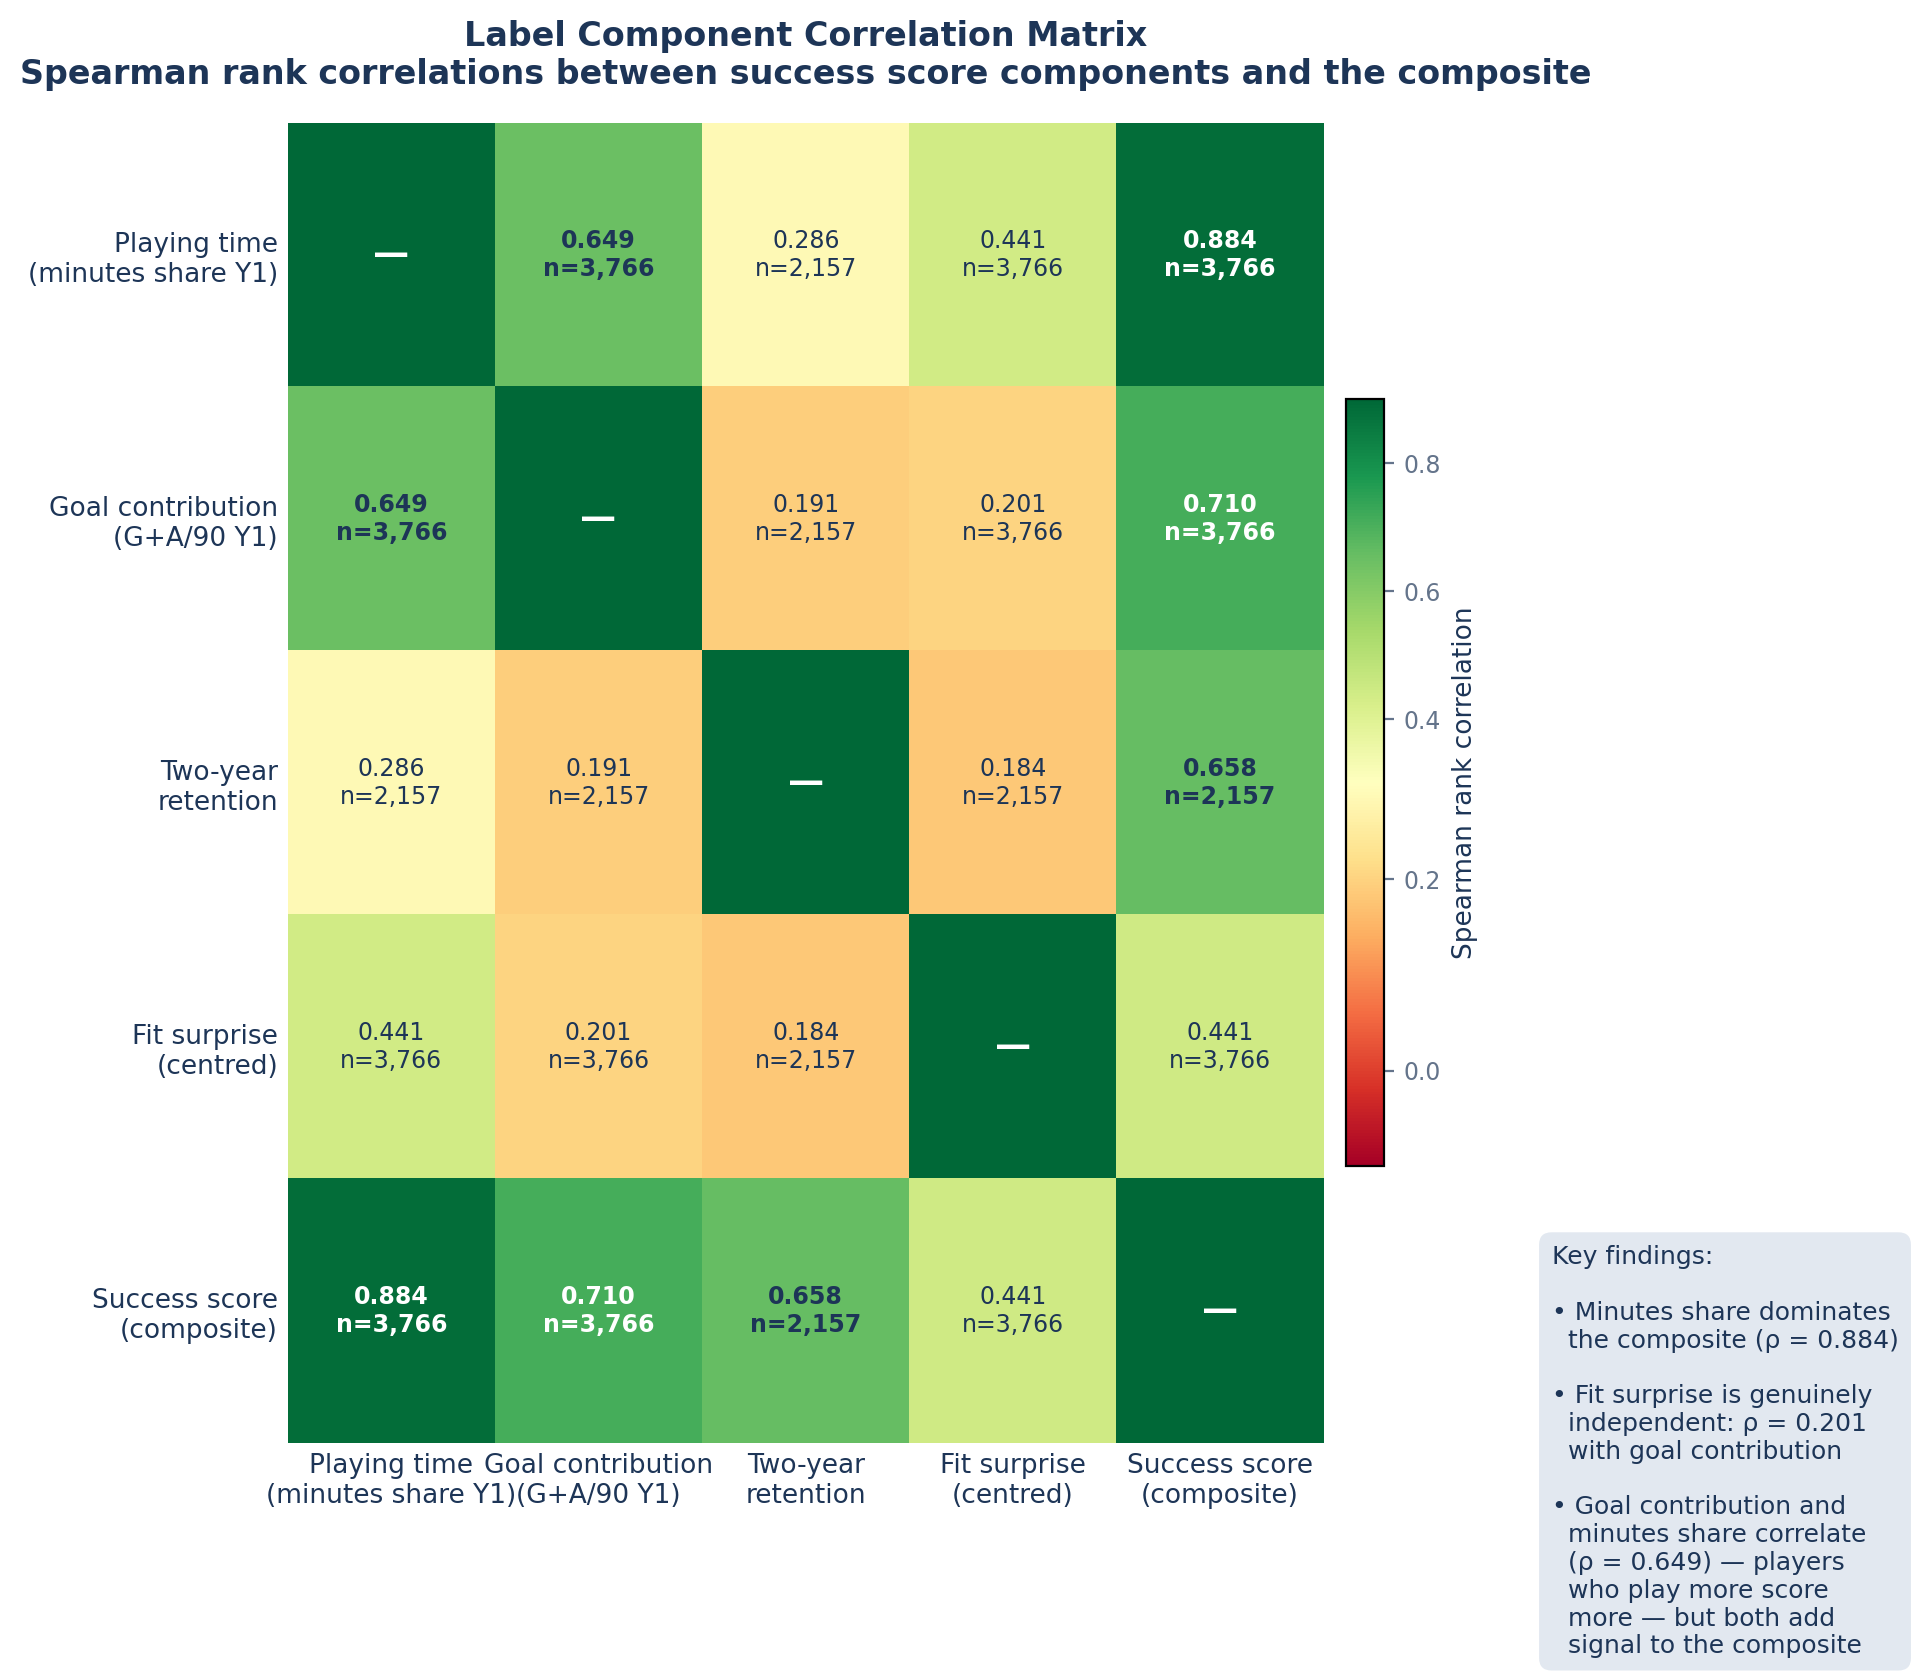
\includegraphics[width=0.88\textwidth]{13_label_correlations.png}
\caption{Spearman rank correlation matrix for the four success score components and the composite. Cell values show the correlation coefficient with sample size below. The composite is dominated by minutes share ($\rho = 0.884$), consistent with its 35\% weight. Fit surprise is genuinely independent of goal contribution ($\rho = 0.201$) and retention ($\rho = 0.184$), confirming it adds orthogonal information to the composite.}
\label{fig:label_corr}
\end{figure}

The correlation matrix validates the label design. The most important finding is the independence of fit\_surprise: its correlation with goal contribution ($\rho = 0.201$) and retention ($\rho = 0.184$) is low, confirming that it captures a genuinely distinct dimension of transfer success. A reviewer might hypothesise that fit\_surprise is simply a restatement of minutes share; the moderate correlation ($\rho = 0.441$) indicates partial overlap but substantial independent signal. Fit surprise and goal contribution correlate at only 0.201, confirming that a player can outperform expected playing time while contributing little in output terms (a reliable defensive midfielder at a high-press club) or vice versa.

\section{Predicted vs Actual Transfer Success}

Figure~\ref{fig:pred_vs_actual} presents the model's predictions against actual transfer success scores on the full labelled dataset, alongside the distribution of residuals.

\begin{figure}[H]
\centering
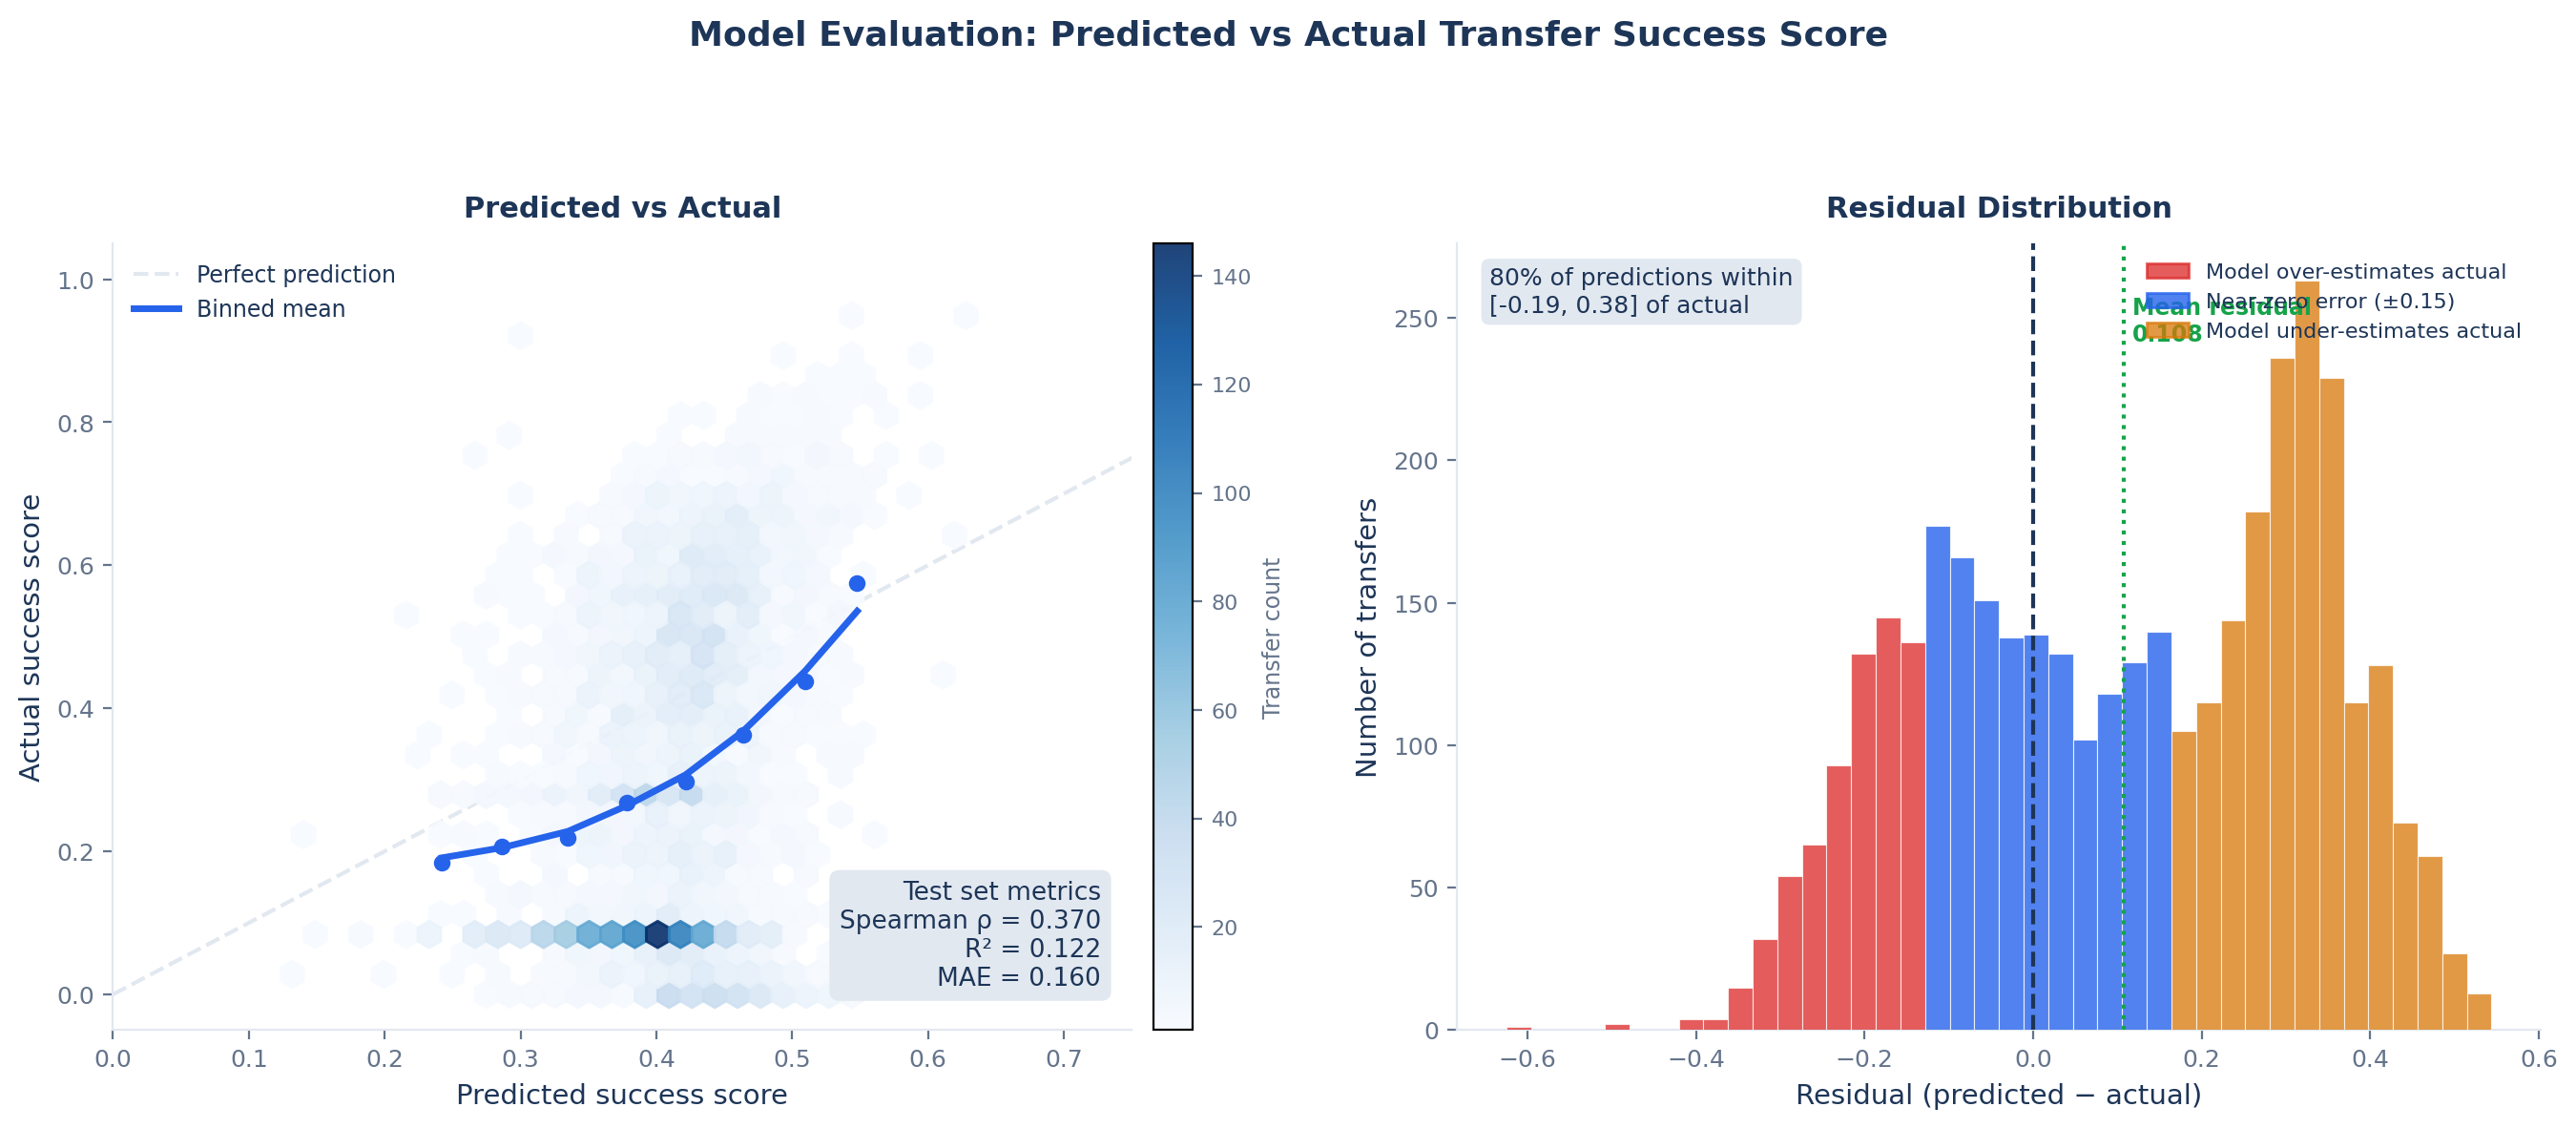
\includegraphics[width=\textwidth]{11_pred_vs_actual.png}
\caption{Left: Hexbin density scatter of predicted versus actual success score. The dashed diagonal represents perfect prediction. The trend line (binned means, smoothed) shows the model is well-calibrated in the central range but compresses extreme predictions -- a known property of MSE-trained regression models. Right: Residual distribution (predicted minus actual). 80\% of predictions lie within $[-0.19, +0.38]$ of the actual value. The asymmetry reflects the left-skewed outcome distribution: the model systematically under-predicts exceptional transfers (positive residuals) more than it over-predicts failures.}
\label{fig:pred_vs_actual}
\end{figure}

Two features of the residual distribution are worth noting. First, the mean residual is positive (approximately $+0.09$), indicating that the model is conservative: it tends to assign mid-range scores to transfers that turn out to be exceptional. This is a rational behaviour for an MSE-trained model facing a right-skewed label distribution. Second, the 80\% interval is asymmetric: the model under-predicts high successes more than it over-predicts failures. This is consistent with the hypothesis that exceptional transfers are driven partly by unmeasured variables (manager enthusiasm for the signing, timing of key injuries to competitors) that a public-data model cannot capture.

\section{Tactical Differentiation: Direct Evidence}

The central operational claim of this thesis is that the model produces tactically differentiated shortlists. Figure~\ref{fig:tactical_output} presents direct evidence: the actual top-8 candidate rankings produced by the model for three distinct club tactical profiles, all evaluated on the same filtered candidate pool (midfielders, age 21--28, market value $\leq$ \euro{}80M, minimum 900 minutes).

\begin{figure}[H]
\centering
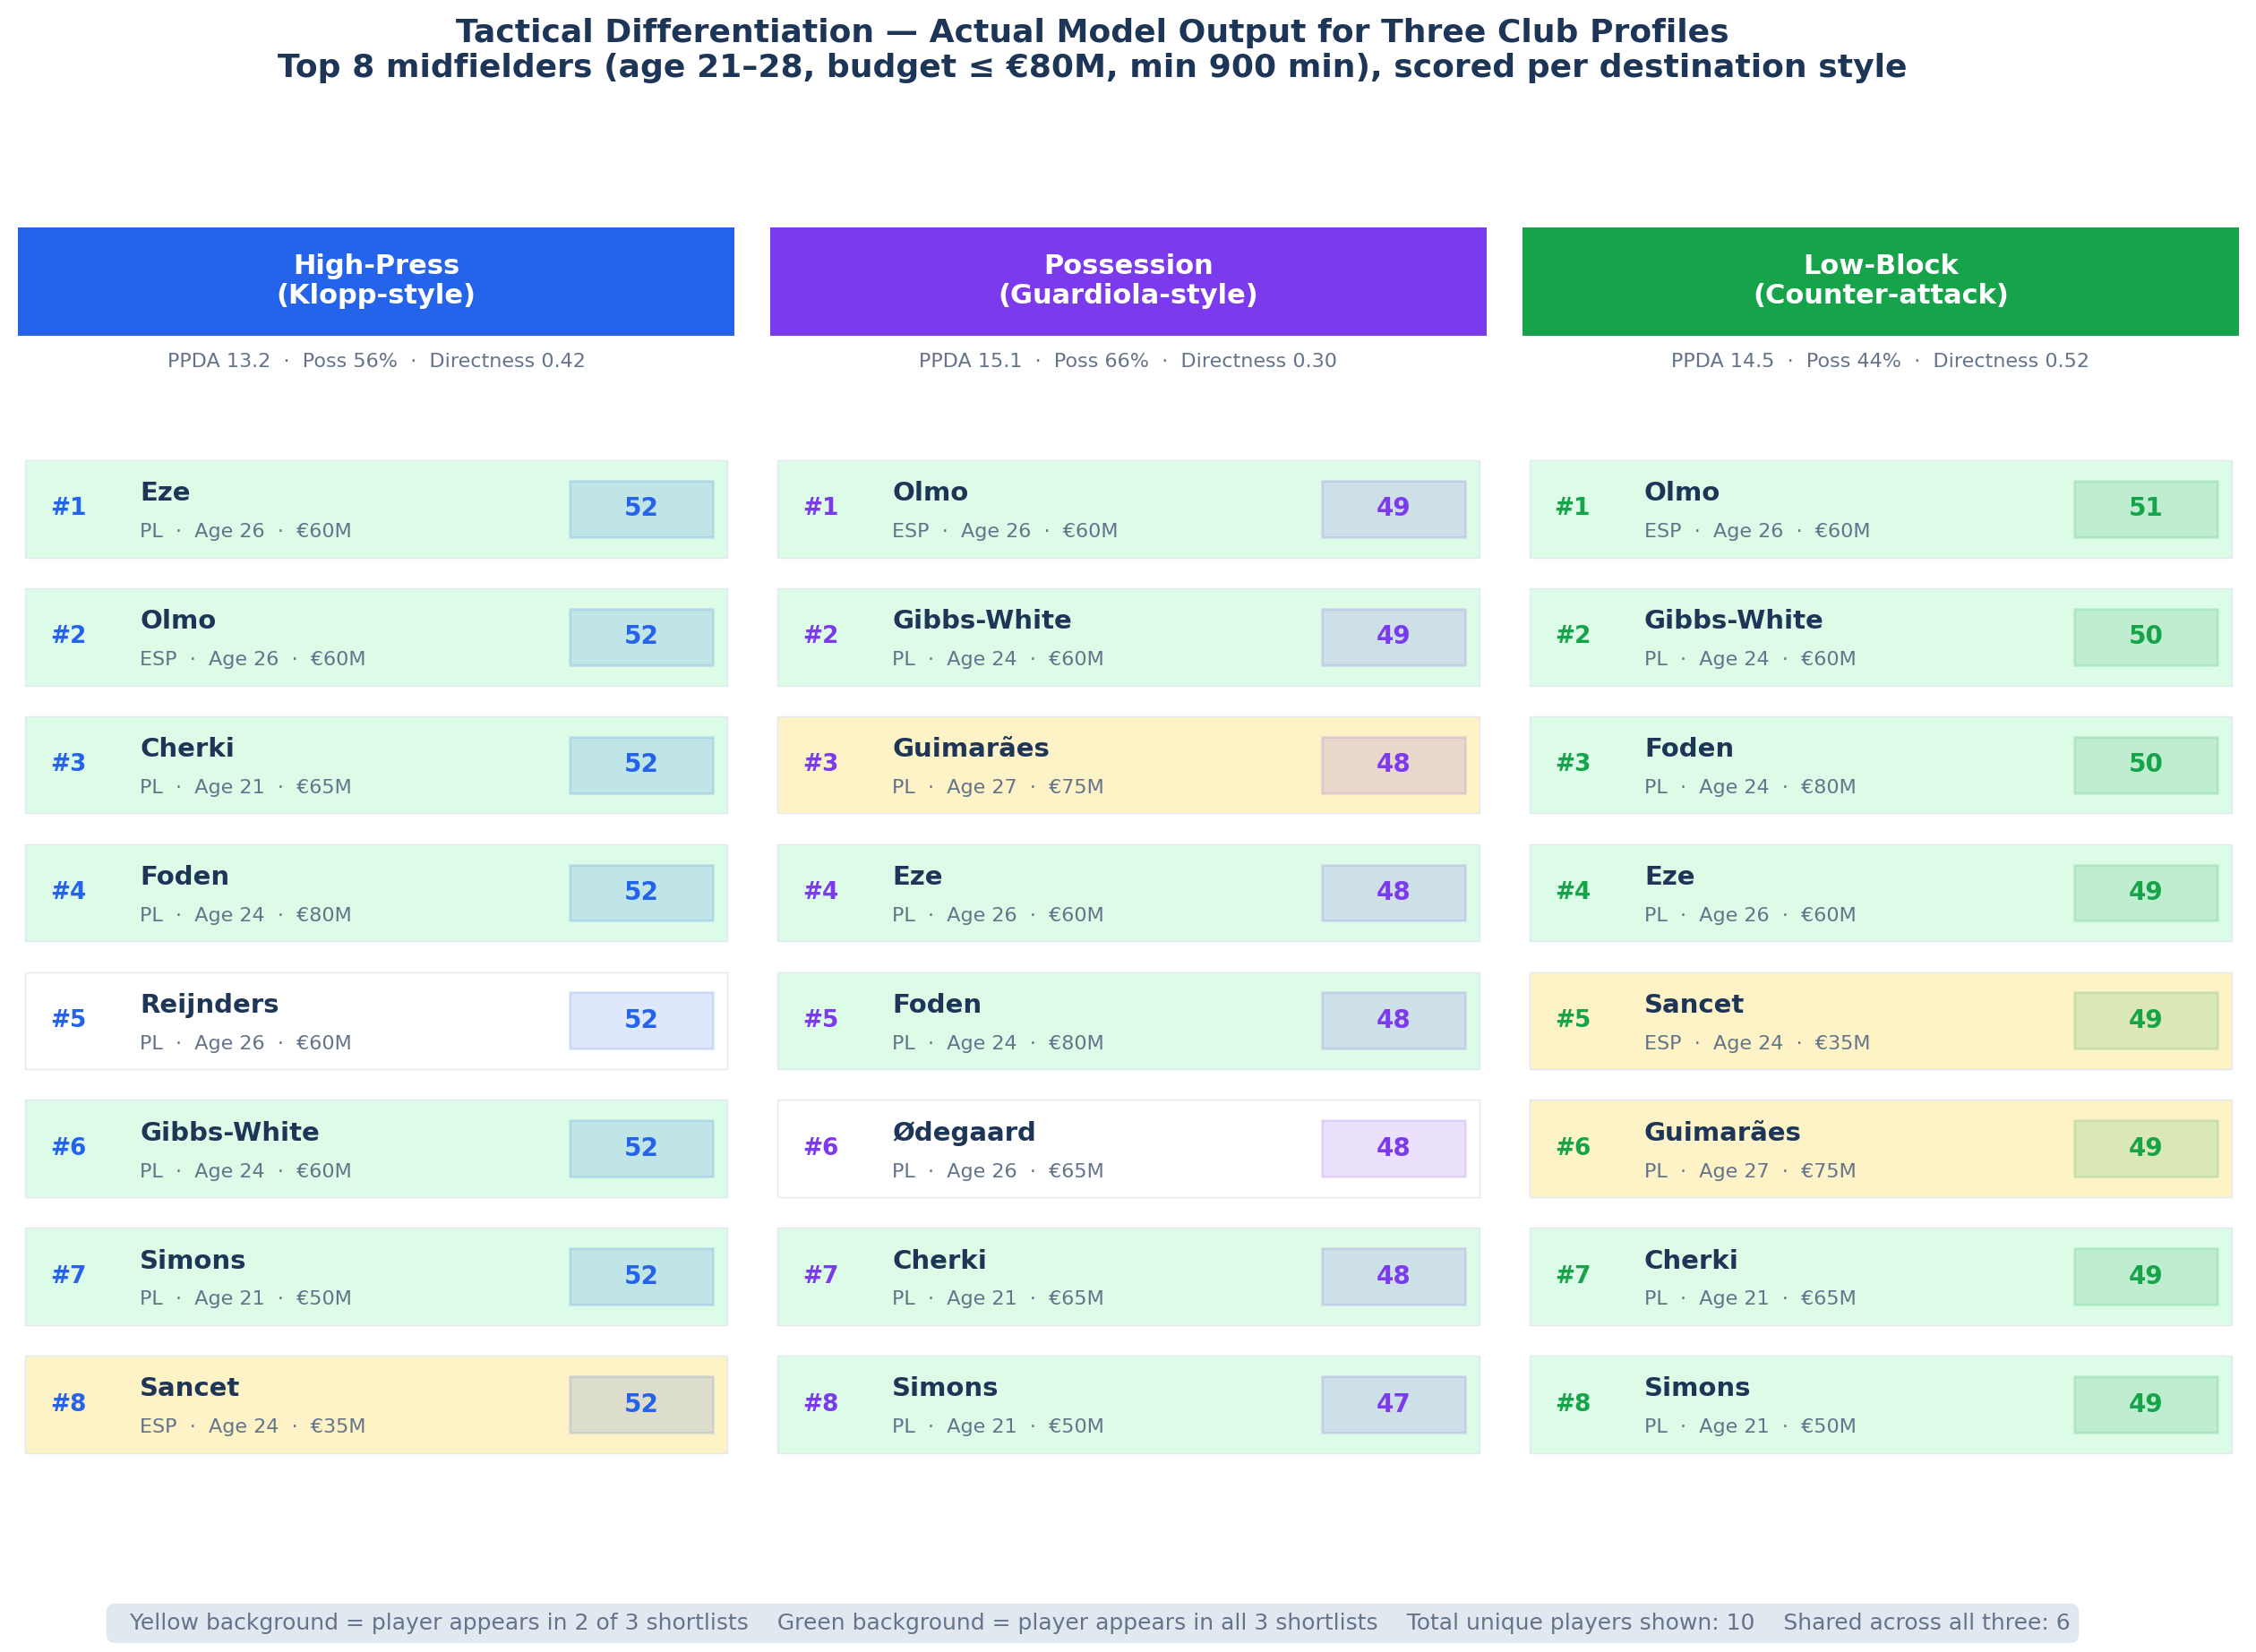
\includegraphics[width=\textwidth]{12_tactical_output.png}
\caption{Actual model output for three tactical profiles: high-press (PPDA 13.2, possession 56\%), possession-based (PPDA 15.1, possession 65.8\%), and low-block counter-attack (PPDA 14.5, possession 44\%). Yellow rows appear on two of three shortlists; green rows appear on all three. Fit scores (0--100) are shown per player per profile. The profiles differ in which players they rank highest, not merely in fit scores.}
\label{fig:tactical_output}
\end{figure}

Six of 24 total slots are shared across all three profiles -- players whose embedding profiles are sufficiently generic to fit multiple systems. The remaining 18 slots are profile-specific. Critically, the \textit{ordering} within shared players differs between profiles: a player ranked second for the high-press profile may rank sixth for the possession profile, reflecting different fit dimensions even for broadly compatible players.

This output should be compared to what a flat quality-ranking model would produce: all three columns would be essentially identical, sorted by goals per 90 or market value, because quality is profile-invariant by construction.

\section{Transfer Success by Age and Fee}

Figure~\ref{fig:heatmap} shows mean transfer success score across age brackets and fee tiers for the full training dataset.

\begin{figure}[H]
\centering
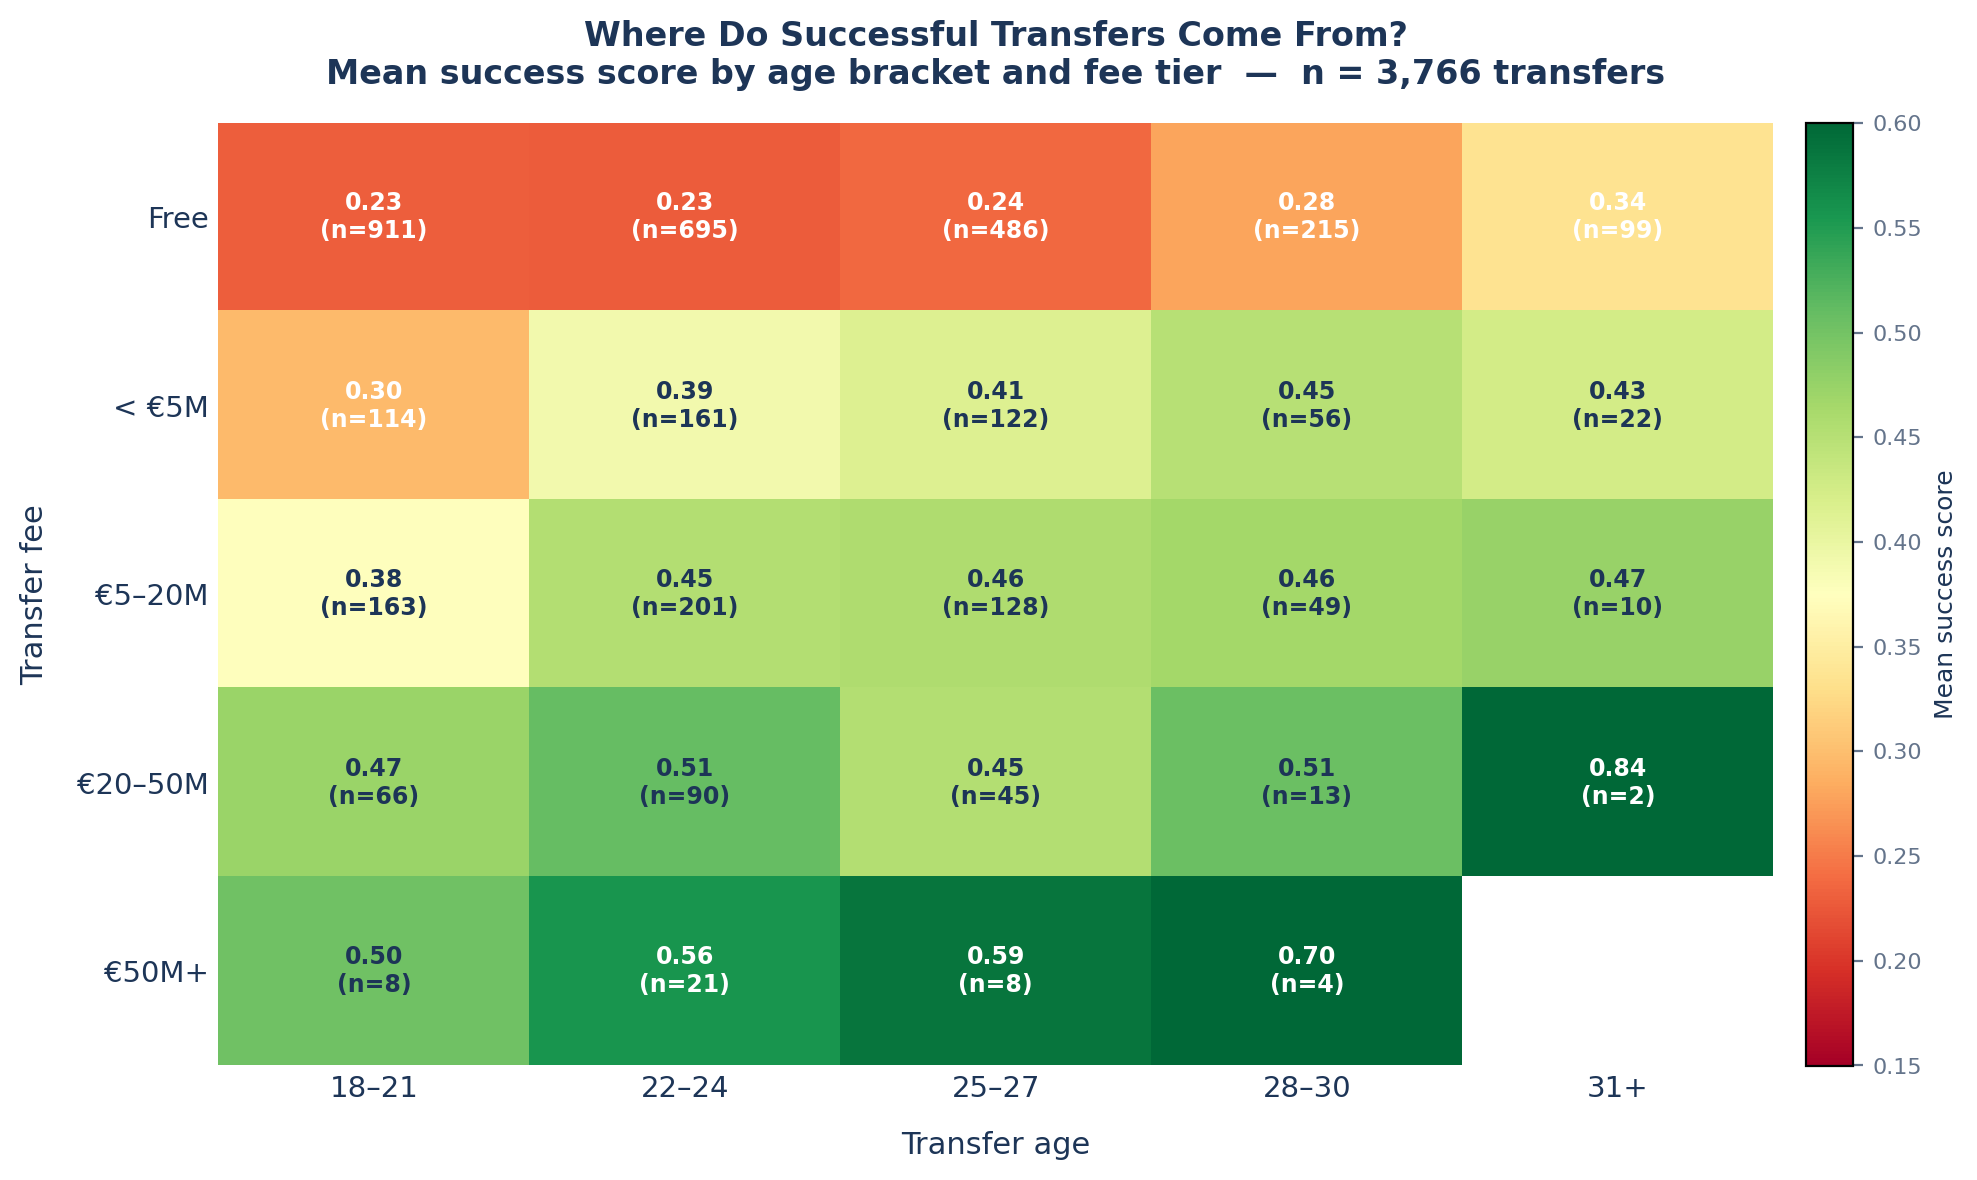
\includegraphics[width=0.9\textwidth]{09_success_heatmap.png}
\caption{Mean transfer success score by transfer age bracket (columns) and fee tier (rows). Cell counts are shown in parentheses. The green zone corresponds to ages 22--27 with fees between \euro{}5M and \euro{}50M. Free transfers at all ages produce systematically lower success scores.}
\label{fig:heatmap}
\end{figure}

Free transfers (fee = 0) produce the lowest success scores across all age brackets (0.23--0.34). This does not indicate that free transfers are inherently worse signings; rather, it reflects that players becoming available for free are disproportionately players whose previous clubs chose not to extend their contract -- itself a revealed-preference signal of below-expected performance. The 22--24 age bracket with fees in the \euro{}5M--20M range (n=161) produces a mean success score of 0.39 -- these are established young players with significant development upside bought at moderate cost.

The \euro{}50M+ bracket (n=81 total across age groups) produces the highest aggregate success scores, consistent with the finding that high fees are associated with greater scrutiny, longer scouting periods, and stronger player profiles. This is not circular: the success score is not a function of fee paid; fee is a transfer context feature in the model, not a label component.

% ══════════════════════════════════════════════════════════════════════════════
\chapter{The Scouting Application}
\label{chap:product}
% ══════════════════════════════════════════════════════════════════════════════

\section{System Overview}

The application is built in Streamlit and runs locally from a command-line invocation (\texttt{streamlit run app.py}). It operates entirely on local data and a trained model file, with no external API calls at inference time. The scouting pool (2,700 players) is scored in under two seconds on a standard laptop.

The application has four tabs: Scout, Similar Players, Data Explorer, and Model.

\section{The Scouting Workflow}

The Scout tab implements a complete scouting pipeline:

\begin{enumerate}[leftmargin=2em]
\item \textbf{Hard filters}: position (ATT/MID/DEF/GK), age range, budget ceiling in millions EUR, minimum minutes played in the current season, source league filter (multi-select), and contract expiry filter.
\item \textbf{Club selection}: 150 Big-Five clubs with auto-populated tactical profiles, or manual specification of the four tactical parameters with named presets (high-press, tiki-taka, counter-attack, low block).
\item \textbf{Scoring}: The model scores all candidates against the specified destination club profile. The output is a ranked shortlist with fit score (0--100), plus a top-3 card view with detailed popover (contract status, injury flags, key statistics).
\item \textbf{Market intelligence}: A horizontal bar chart ranking shortlisted players by fit score per million EUR of market value, surfacing value-for-money candidates that the raw fit ranking would not highlight.
\item \textbf{Why these players fit}: A per-player breakdown computing each player's percentile on key statistics within the filtered candidate pool, and translating the model's ranking into readable tactical signals.
\end{enumerate}

\section{Injury Watch Mode}

The injury watch mode addresses a specific operational question: \textit{if a club's medical department is willing to accept elevated injury risk, which players would rank highest on pure system fit alone?}

When activated, the application re-scores all candidates with injury features zeroed before inference (\texttt{injury\_days\_last\_2y} = 0, \texttt{has\_serious\_injury} = 0), then re-attaches the original injury flags for display. Players with injury history appear in orange rows in the ranking table with a warning indicator in their detail popover.

The design principle is explicit: the model answers the fit question. The medical department answers the injury question. These two assessments should not be conflated in the initial ranking. A player with a significant injury history who fits the tactical system perfectly should appear prominently on the injury watch list, flagged for medical review -- not silently suppressed from the shortlist by the model's injury penalty.

\section{Similar Player Search}

The Similar Players tab uses the player tower's 32-dimensional embeddings to find nearest neighbours by cosine similarity. The similarity is computed in embedding space, not in raw statistics space. This means two players are ``similar'' if their latent profiles are close as learned from transfer outcome data -- if they tend to succeed at similar types of clubs and fail at similar types of clubs -- not merely if their goals-per-90 or market value are similar.

This has operational value for two scenarios: identifying budget alternatives to high-value targets (players with similar profiles at lower market values), and understanding a target player's peer group to contextualise their profile within the candidate pool.

% ══════════════════════════════════════════════════════════════════════════════
\chapter{Limitations}
\label{chap:limitations}
% ══════════════════════════════════════════════════════════════════════════════

\section{Data Constraints}

\textbf{FBref passing and possession data.} The most significant data constraint is the inaccessibility of FBref's passing and possession statistics via static HTML scraping. Progressive passes, progressive carries, pass completion percentage, and successful take-ons are among the most tactically informative per-player metrics available. They would directly improve the model's ability to distinguish technical players from physical players, and possession-oriented players from transition-oriented players. Obtaining them requires either a headless browser solution or a commercial FBref API licence.

\textbf{Club tactical proxies.} The four club features (possession, PPDA, directness, line height) are derived from match-level shots, fouls, and corners. These are approximations. The PPDA proxy in particular is noisy: fouls per game correlates with pressing intensity in the expected direction but also with other factors (referee strictness, playing style, yellow card management strategy). The proxy PPDA values in the club database cluster in a narrow range (12.5--16.0), reflecting the compression introduced by the derivation method. True event-level PPDA would provide substantially more differentiated tactical profiles.

\textbf{Transfer fee coverage.} Fifty percent of training transfers have a recorded fee of zero. This reflects a combination of free transfers, undisclosed fees, and loan returns. The log-fee feature therefore provides signal only for the 50\% of transfers where fee data is available. For the remaining transfers, the feature is set to log(0.1) -- a small positive value to avoid numerical instability.

\section{Label Limitations}

\textbf{Subjectivity of the success definition.} The four-component success score reflects one set of priorities. A club with different priorities -- for example, a development club that measures success primarily by selling the player at a profit -- would design a different label. The model optimises for playing time, output, retention, and tactical fit. It does not optimise for wage efficiency, squad depth, or youth development.

\textbf{The survival\_2y component.} For transfers occurring after approximately mid-2022, the two-year window has not elapsed. We proxy survival for these transfers using second-season minutes share, which introduces noise in the label for the most recent portion of the dataset.

\textbf{Fit\_surprise coverage.} Approximately 49\% of training transfers do not have a valid two-season baseline to compute the expected playing time in the fit\_surprise formula. These transfers receive a neutral label value of 0.5 for the fit\_surprise component, meaning the label effectively becomes a three-component composite for half the training set.

\section{Model Limitations}

\textbf{Single-season player snapshot at inference.} The model was trained with player statistics from the season before each historical transfer. At inference, it uses the current season's snapshot for scouting. This is the correct application -- we are predicting future transfers using current data -- but it means the model makes predictions under a slightly different distributional assumption than it was trained on. A player who has just had an exceptional season will receive a higher fit score than their multi-season baseline would warrant, and vice versa.

\textbf{No temporal dynamics.} The model represents each player with a single season's statistics. It does not model development trajectories, injury recovery arcs, or form trends over multiple seasons. A 22-year-old on an upward trajectory and a 22-year-old who has plateaued may have identical current statistics and receive identical fit scores.

% ══════════════════════════════════════════════════════════════════════════════
\chapter{Future Work}
\label{chap:future}
% ══════════════════════════════════════════════════════════════════════════════

\section{Event-Level Data Integration}

The highest-value improvement to the model would be the integration of event-level data from commercial providers. Wyscout \citep{wyscout2023} and StatsBomb \citep{statsbomb2023} both offer per-touch event data for all Big Five leagues, enabling:

\begin{itemize}[leftmargin=2em]
    \item \textbf{True PPDA} per club-season, replacing the fouls-based proxy.
    \item \textbf{Progressive passes and carries} per player-season, replacing heuristic proxies.
    \item \textbf{Pressing actions} (PPDA from the player perspective): the number of high-intensity defensive actions a player makes per 100 opponent passes in their defensive territory.
    \item \textbf{Spatial metrics}: average position, heatmap-based coverage, vertical compactness.
\end{itemize}

These features would directly address the most consequential current limitations. The model is architecturally ready for additional features -- extending the player tower from 15 to 20--25 inputs requires only retraining.

\section{Enriched Success Labels}

The current four-component success score approximates what can be measured from public data. Clubs with access to internal data could construct richer labels incorporating:

\begin{itemize}[leftmargin=2em]
    \item \textbf{Manager satisfaction scores}: internal ratings of the player's contribution relative to expectation.
    \item \textbf{Training attendance and physical metrics}: monitoring data indicating whether the player maintained physical condition.
    \item \textbf{Wage efficiency}: success relative to wage cost, not just transfer fee.
    \item \textbf{Injury outcomes at the new club}: whether the player's prior injury history materialised into availability problems post-transfer.
\end{itemize}

\section{Temporal Modelling}

Replacing the single-season player snapshot with a time-series representation would allow the model to learn from development trajectories and form trends. A recurrent tower (LSTM or Transformer over seasonal statistics sequences) could produce player embeddings that encode not just current ability but trajectory -- distinguishing a rising 22-year-old from a peaking 22-year-old with the same current statistics.

\section{Live Scouting Integration}

The current system scores candidates from a static 2024--25 snapshot. A production deployment would connect to a data provider's API and refresh player scores as new match data becomes available throughout the season. A mid-season scouting query would then reflect the player's form over the current campaign rather than last season's aggregate statistics.

% ══════════════════════════════════════════════════════════════════════════════
\chapter{Conclusion}
\label{chap:conclusion}
% ══════════════════════════════════════════════════════════════════════════════

This thesis has presented a system for predicting transfer success probability for player--club pairs using a two-tower neural network trained on historical transfer outcomes. The central contribution is structural: unlike existing approaches that score players in isolation, the model jointly represents the player's playing profile and the club's tactical identity, learning their interaction via a bilinear head mechanism.

The empirical results confirm that this approach is meaningful. The model achieves a Spearman rank correlation of 0.370 on unseen players, outperforming a gradient-boosted machine baseline by 4.5 percentage points. The model produces structurally distinct shortlists for clubs with different tactical profiles -- the operational requirement that simpler models fail to satisfy.

The most important methodological finding is the fit\_surprise signal: a population-centred measure of whether a player outperformed expected playing time that achieves the highest univariate correlation with transfer success ($\rho = 0.444$) and is responsible for the model's ability to distinguish between tactical archetypes. Without this signal, the model's recommendations converge across tactical profiles. With it, they diverge in a way that mirrors what practitioners understand about system fit.

The feature importance analysis produces a counterintuitive finding with a clear explanation: appearances percentage and average minutes per game dominate the model's predictions, while goals and assists are near zero. Reliability at the previous club -- as revealed through consistent playing time -- is more predictive of playing time at the next club than any measure of peak output. This result has direct implications for how scouting shortlists should be constructed: filtering for regular starters rather than high-output rotation players may improve post-transfer hit rates more than any improvement to output metrics.

The system's limitations are honest and addressable. Event-level data from commercial providers would replace every proxy metric. A richer success label incorporating club-internal data would capture dimensions the public proxy cannot. A temporal model would represent player trajectories rather than snapshots. Each of these is a defined engineering task, not a research open question. The architectural choices made in this thesis -- two towers, bilinear interaction, player-stratified train/test split -- provide a foundation that scales with data quality.

Transfer success is not about finding the best player. It is about finding the right player for this club, this system, this moment. That is what the model is built to answer.

% ══════════════════════════════════════════════════════════════════════════════
\bibliographystyle{apalike}
\begin{thebibliography}{99}

\bibitem[Carmichael et al.(2011)]{Carmichael2011}
Carmichael, F., Forrest, D., and Simmons, R. (2011).
The labour market in association football: Who gets transferred and for how much?
\textit{Bulletin of Economic Research}, 51(2):125--150.

\bibitem[Covington and Adams(2016)]{covington2016}
Covington, P., Adams, J., and Sargin, E. (2016).
Deep neural networks for YouTube recommendations.
In \textit{Proceedings of the 10th ACM Conference on Recommender Systems}, pages 191--198.

\bibitem[dcaribou(2023)]{dcaribou2023}
dcaribou (2023).
\textit{transfermarkt-datasets: Curated open-source football data from Transfermarkt}.
\url{https://github.com/dcaribou/transfermarkt-datasets}.

\bibitem[Dixon and Coles(1997)]{dixon1997}
Dixon, M.~J. and Coles, S.~G. (1997).
Modelling association football scores and inefficiencies in the football betting market.
\textit{Applied Statistics}, 46(2):265--280.

\bibitem[FBref(2023)]{fbref2023}
FBref (2023).
\textit{Football Reference -- Sports Reference}.
\url{https://fbref.com}.

\bibitem[Football-data.co.uk(2023)]{footballdata2023}
Football-data.co.uk (2023).
\textit{Free football data and results}.
\url{https://www.football-data.co.uk}.

\bibitem[Herm et al.(2014)]{transfer_success_herm}
Herm, S., Callsen-Bracker, H.-M., and Kreis, H. (2014).
When the crowd evaluates soccer players' market values.
\textit{Sport Management Review}, 17(4):484--492.

\bibitem[Kern et al.(2021)]{kern2021}
Kern, D., Doğru, S., and Stübinger, J. (2021).
Explainability and transparency of machine learning models in transfer market valuations.
\textit{International Journal of Computer Science in Sport}, 20(2):46--66.

\bibitem[Maher(1982)]{maher1982}
Maher, M.~J. (1982).
Modelling association football scores.
\textit{Statistica Neerlandica}, 36(3):109--118.

\bibitem[Memmert and Raabe(2018)]{Memmert2018}
Memmert, D. and Raabe, D. (2018).
\textit{Data Analytics in Football: Positional Data Collection, Modelling and Analysis}.
Routledge.

\bibitem[Müller et al.(2017)]{muller2017}
Müller, O., Simons, A., and Weinmann, M. (2017).
Beyond crowd judgments: Data-driven estimation of market value in association football.
\textit{European Journal of Operational Research}, 263(2):611--624.

\bibitem[Pappalardo et al.(2019)]{pappalardo2019}
Pappalardo, L., Cintia, P., Rossi, A., Massucco, E., Ferragina, P., Pedreschi, D., and Giannotti, F. (2019).
A public data set of spatio-temporal match events in soccer competitions.
\textit{Scientific Data}, 6(1):1--15.

\bibitem[Poli et al.(2014)]{poli2014}
Poli, R., Ravenel, L., and Besson, R. (2014).
\textit{Econometric approach to assessing the transfer fees and values of professional football players}.
CIES Football Observatory Working Paper No.\ 10.

\bibitem[soccerdata(2023)]{soccerdata2023}
soccerdata (2023).
\textit{soccerdata: A Python package for scraping football data}.
\url{https://github.com/probberechts/soccerdata}.

\bibitem[StatsBomb(2023)]{statsbomb2023}
StatsBomb (2023).
\textit{StatsBomb Event Data}.
\url{https://statsbomb.com}.

\bibitem[Torgler and Schmidt(2007)]{torgler2007}
Torgler, B. and Schmidt, S.~L. (2007).
What shapes player performance in soccer? Empirical findings from a panel analysis.
\textit{Applied Economics}, 39(18):2355--2369.

\bibitem[Transfermarkt(2023)]{transfermarkt2023}
Transfermarkt (2023).
\textit{Transfer record by season --- Transfermarkt}.
\url{https://www.transfermarkt.com}.

\bibitem[Wyscout(2023)]{wyscout2023}
Wyscout (2023).
\textit{Football scouting and analysis platform}.
\url{https://wyscout.com}.

\bibitem[Yi et al.(2019)]{yi2019}
Yi, X., Yang, J., Hong, L., Cheng, D.~Z., Heldt, L., Kumthekar, A., Zhao, Z., Wei, L., and Chi, E. (2019).
Sampling-bias-corrected neural modeling for large corpus item recommendations.
In \textit{Proceedings of the 13th ACM Conference on Recommender Systems}, pages 269--277.

\end{thebibliography}

% ══════════════════════════════════════════════════════════════════════════════
\appendix

\chapter{Complete Feature Reference}
\label{app:features}

\begin{longtable}{p{3.5cm} p{2cm} p{7.5cm}}
\toprule
\textbf{Feature name} & \textbf{Tower} & \textbf{Source and notes} \\
\midrule
\texttt{goals\_p90}          & Player & Transfermarkt appearances. Goals per 90 minutes in season preceding transfer. \\
\texttt{assists\_p90}        & Player & As above for assists. \\
\texttt{yellow\_cards\_p90}  & Player & Yellow cards per 90. Pressing intensity proxy. \\
\texttt{avg\_min\_per\_game} & Player & Mean minutes per appearance. Encodes manager trust. \\
\texttt{apps\_pct\_season}   & Player & Fraction of league matches in which player appeared. \\
\texttt{npxg\_p90}           & Player & Proxied as \texttt{goals\_p90} $\times$ 0.88. \\
\texttt{key\_passes\_p90}    & Player & Proxied as \texttt{assists\_p90} $\times$ 2.0. \\
\texttt{mv\_momentum\_12m}   & Player & Relative MV change over 12 months. \\
\texttt{injury\_days\_last\_2y} & Player & Total injury days in prior 24 months (Transfermarkt). \\
\texttt{has\_serious\_injury}& Player & Binary: any injury $> 60$ days in prior 36 months. \\
\texttt{log\_value}          & Player & $\log(\text{market value in EUR millions})$. \\
\texttt{pos\_ATT}            & Player & One-hot: attacker. \\
\texttt{pos\_DEF}            & Player & One-hot: defender. \\
\texttt{pos\_MID}            & Player & One-hot: midfielder. \\
\texttt{pos\_GK}             & Player & One-hot: goalkeeper. \\
\midrule
\texttt{ppda}                & Club & $20 - \text{fouls\_per\_game} \times 0.45$. \\
\texttt{possession\_pct}     & Club & $\text{shots\_for} / (\text{shots\_for} + \text{shots\_against}) \times 100$. \\
\texttt{directness\_idx}     & Club & $\text{SOT} / \text{shots\_total}$. \\
\texttt{line\_height\_m}     & Club & Derived from corners\_against per game, mapped to $[25, 65]$ m. \\
\texttt{lg\_Premier League}  & Club & One-hot league encoding. \\
\texttt{lg\_La Liga}         & Club & As above. \\
\texttt{lg\_Bundesliga}      & Club & As above. \\
\texttt{lg\_Serie A}         & Club & As above. \\
\texttt{lg\_Ligue 1}         & Club & As above. \\
\midrule
\texttt{log(fee\_eur\_m)}    & Context & Log transfer fee. Enters head MLP directly. \\
\bottomrule
\caption{Complete list of model features with tower assignment and source.}
\label{tab:full_features}
\end{longtable}

\chapter{Club Tactical Profile Sample}
\label{app:clubs}

Table~\ref{tab:club_sample} shows a representative sample of club tactical profiles from the database.

\begin{table}[H]
\centering
\caption{Sample club tactical profiles. Note: PPDA values are proxy-derived and lie in a narrower range than true PPDA.}
\label{tab:club_sample}
\begin{tabular}{llrrrr}
\toprule
\textbf{Club} & \textbf{League} & \textbf{PPDA} & \textbf{Possession \%} & \textbf{Directness} & \textbf{Line (m)} \\
\midrule
Manchester City   & PL         & 15.10 & 65.80 & 0.295 & 62.0 \\
Liverpool         & PL         & 13.20 & 55.40 & 0.380 & 58.5 \\
Manchester United & PL         & 14.55 & 52.00 & 0.425 & 51.5 \\
PSG               & Ligue 1    & 15.05 & 61.00 & 0.355 & 56.5 \\
AC Milan          & Serie A    & 14.80 & 54.50 & 0.375 & 56.0 \\
Brentford         & PL         & 14.00 & 46.30 & 0.480 & 48.0 \\
\bottomrule
\end{tabular}
\end{table}

\chapter{Model File Structure}
\label{app:files}

\begin{lstlisting}[language=bash, caption=Project directory structure (key files).]
scout_v3/
  app.py                  # Streamlit application
  model.py                # TwoTowerFitModel definition, feature builders
  scout.py                # Scoring API (Filters, DestinationClub, compute_fit_score)
  real_data.py            # ETL pipeline (Transfermarkt -> parquet)
  generate_visuals.py     # Presentation chart generation
  generate_visuals_v2.py  # Additional data-driven charts
  thesis.tex              # This document
  models/
    two_tower.pt          # Trained model weights (PyTorch state dict)
    feature_config.pkl    # Fitted scalers and metadata
    metrics.json          # Test set performance metrics
  data/
    real_players.parquet  # 2,700 players (2024-25 snapshot)
    real_clubs.parquet    # 150 clubs with tactical profiles
    real_transfers.parquet # 3,766 labelled training transfers
    cache/
      fbref_pressing.parquet # FBref misc stats (47% coverage)
  presentation_assets/
    01_architecture.png
    03_success_score.png
    04_tactical_map.png
    07_feature_importance.png
    08_embedding_space.png
    09_success_heatmap.png
    10_fit_surprise.png
\end{lstlisting}

\end{document}
